\documentclass[a4paper]{report}

\usepackage{cmap}
\usepackage[utf8]{inputenc}
\usepackage{graphbox}
\usepackage{float}
\usepackage{hyperref}
\usepackage{wrapfig}
\usepackage[italian]{babel}
\usepackage{multicol}
\usepackage{titlesec}
\usepackage{tabu}
\usepackage{fix-cm}
\usepackage[margin=2cm]{geometry}
\usepackage[pages=some]{background}
\usepackage{listings}
\usepackage{tcolorbox}
\usepackage{pdfpages}
\graphicspath{ {images/} }

% Cambio il nome ai titoletti 
\renewcommand{\chaptername}{Capitolo}
\renewcommand{\contentsname}{Contenuti}
\renewcommand{\abstractname}{}
\renewcommand{\bibname}{Bibliografia}
\renewcommand{\figurename}{Figura}
\renewcommand{\tablename}{Tabella}

% Regole di formattazione
\newcommand\tstrut{\rule{0pt}{2.4ex}}
\newcommand\bstrut{\rule[-1.0ex]{0pt}{0pt}}
\newcolumntype{P}[1]{>{\centering\arraybackslash}p{#1}}
\setlength\parindent{0pt}
\newcommand{\setuptext}{
\fontsize{12}{14}\selectfont
\setlength{\parskip}{0.4cm}
\titlespacing{\section}{0pt}{*2}{*0}
}

% Definisco il titolone
\makeatletter
\newcommand\HUGE{\@setfontsize\Huge{50}{60}}
\makeatother   

% Definisco i Riquadri colorati
\definecolor{darkgreen}{rgb}{0.000, 0.392, 0.000}
\definecolor{darkred}{rgb}{0.502, 0.000, 0.000}
\newenvironment{ricordati}{\begin{tcolorbox}[fonttitle=\sffamily\bfseries\large,title=Ricordati,colframe=orange!75!white]}{\end{tcolorbox}}
\newenvironment{info}{\begin{tcolorbox}[fonttitle=\sffamily\bfseries\large,title=Info,colframe=blue!75!white]}{\end{tcolorbox}}
\newenvironment{funzioni}{\begin{tcolorbox}[fonttitle=\sffamily\bfseries\large,title=Funzioni Utili,colframe=darkgreen!75!white]}{\end{tcolorbox}}
\newenvironment{pattern}{\begin{tcolorbox}[fonttitle=\sffamily\bfseries\large,title=Pattern Ricorrenti,colframe=darkred!75!white]}{\end{tcolorbox}}
\newenvironment{code}{\begin{tcolorbox}[size=small]}{\end{tcolorbox}}

% Imposto il Syntax Highlighting
\lstset{
	language=bash
}
\lstset{
	morekeywords={man,ls,cd,pwd,df,du,rm,cp,mv,ln,mkdir,rmdir,sort,head,tail,find,ip,sudo,ifup,systemctl,grep,egrep}
}
\lstset{basicstyle=\ttfamily,
	showstringspaces=false,
	commentstyle=\color{red},
	keywordstyle=\color{blue},
}

% Invoco lo script python per generare automaticamente gli snippet
% RICORDARSI DI ABILITARE L'OPZIONE: -enable-write18
\immediate\write18{python ./snippetbuilder.py}

\begin{document}
	
% COPERTINA
	
\begin{titlepage}
	\centering
	
	\large
	A cura di Federico Terzi e Massimo Schembri - Ultima revisione: \today
	
	\noindent\rule{15cm}{0.2pt}
	
	\vspace{4cm}
	
	\HUGE
	\textbf{LAS}
	
	\huge
	Guida pratica per l'esame di laboratorio
	
	\vspace{2cm}
	
	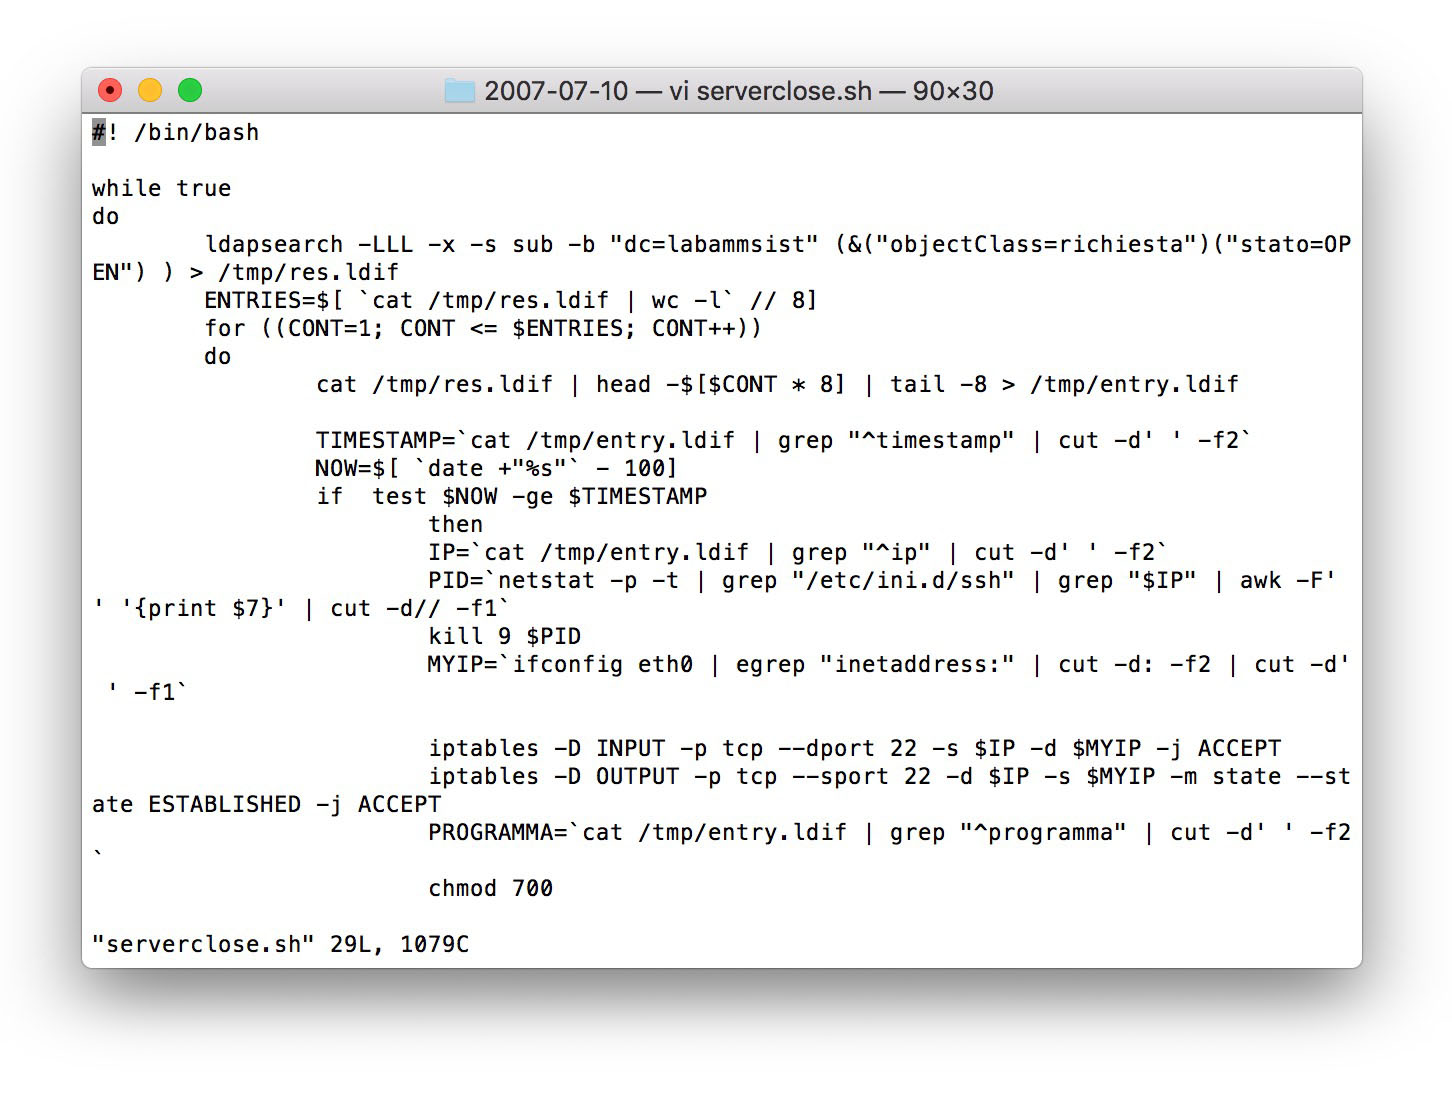
\includegraphics[width=0.9\linewidth]{cover}
	
	\vspace{3cm}
	
	\normalsize
	\url{https://github.com/federico-terzi/las-guida-pratica}
	
	\clearpage
\end{titlepage}

% INTRODUZIONE

\renewcommand{\abstractname}{}
\begin{abstract}
	\section*{Introduzione}
	Ho deciso di scrivere questa guida per unire una miriade di appunti sparsi trovati in rete, nelle slide e in laboratorio in modo da rendere più facile il superamento dell'esame di LAS.

	Pur non essendo esaustiva in ogni aspetto, la guida parla della maggior parte delle tematiche affrontate in laboratorio, soffermandosi sui problemi più comuni.
		
	\section*{Contribuire alla guida}
	
	Se ritieni di poter migliorare la guida o hai trovato un errore, visita la repository GitHub ed apri una \textit{issue}, oppure inviami un messaggio. Ogni contributo è ben accetto :)
	
	\vspace{4mm}
	Link Repository: \url{https://github.com/federico-terzi/las-guida-pratica}
	
	\vspace{5mm}
	
	\begin{figure}[htb!]
		\centering
		
\includegraphics[width=4cm]{qr}
		\caption{QR Code alla repository di GitHub}
	\end{figure}

	\section*{Fonti}
	\begin{itemize}
		\item Molto materiale è tratto dalle slide del Prof. Marco Prandini che sono liberamente disponibili a questo indirizzo: \url{http://lia.disi.unibo.it/Courses/AmmSistemi1718/}
		\item Il \textit{cheat sheet} regex alla fine è tratto dal sito: \url{http://addedbytes.com}
	\end{itemize}
\end{abstract}


% INDICE 
\normalsize
\tableofcontents

% Define the automatic title link button
\titleformat{\section}[hang]{\normalfont\Large\bfseries}{\thesection }{1em}{\addlink}
\titleformat{\subsection}[hang]{\normalfont\large\bfseries}{\thesubsection }{1em}{\addlink}
\newcommand{\addlink}[1]{#1 \href{./snippets/\thesubsection.txt}{
\includegraphics[ width=0.4cm]{open}}}



\chapter{Linguaggio Bash}

\section{Variabili speciali}

All'interno di uno script bash è possibile utilizzare una serie di variabili built-in:

\begin{table}[h]
	\centering
	\begin{tabular}{ll}
		\$\$   & PID dello script bash corrente \\
		\$\#   & Numero di argomenti da riga di comando                                                                                                                                                                                                                                                                                                                                                                                                       \\
		\$?    & Exit value dell'ultimo comando eseguito command.                                                                                                                                                                                                                                                                                                                                                                                                       \\
		\$     & PID della shell                                                                                                                                                                                                                                                                                                                                                                                                       \\
		\$!    & PID dell'ultimo comando eseguito in background                                                                                                                                                                                                                                                                                                                                                                                           \\
		\$0    & Nome script search.                                                                                                                                                                                                                                                                                                                                 \\
		\$n    & N-esimo argomento posizionale. Il massimo numero è 9 \\
		\$*, \$@ & Tutti gli argomenti passati.                                                                                                                                                                                                                                                                                                                                                                                              \\
		"\$*"  & Tutti gli argomenti in un unica stringa "\$1 \$2 ...". I valori sono separati da \$IFS.      \\
		"\$@"  & Tutti gli argomenti, separati individualmente ("\$1" "\$2" …).                                                                                                                                                                                                                                                                                                                                                                         
	\end{tabular}
\end{table}

\section{Escaping degli apici}

Nella shell bash, i singoli apici e i doppi apici assumo significati particolari e ben distinti:

\begin{itemize}
\item \textbf{Singoli apici:} Preservano tutto il contenuto, senza effettuare alcuna valutazione.
\item \textbf{Doppi apici:} Preservano il contenuto, ad eccezione dei caratteri: \texttt{\$, `, \textbackslash, !} che vengono invece interpretati. 
\end{itemize}

\begin{code}
\begin{lstlisting}
USER=pippo
echo "Ciao $USER"   # Stampa: Ciao pippo
echo 'Ciao $USER'   # Stampa: Ciao $USER
echo "$(echo ciao)" # Stampa: ciao
echo '$(echo ciao)' # Stampa: $(echo ciao)
\end{lstlisting}
\end{code}

\begin{info}
Un interessante proprietà degli apici è che possono essere concatenati in un unica stringa. Questo può essere molto utile per formare argomenti che includono variabili esterne ma che vanno anche protetti.

\begin{lstlisting}
echo "ciao"'ciao'             # Stampa: ciaociao

USER=pippo
echo "ciao $USER"'ciao $USER' # Stampa: ciao pippociao $USER

# Esempio un po' piu complesso:
ssh "$1" "echo $2 $3 > "'/tmp/$(echo $SSH_CLIENT | cut -f1 -d" ")'
\end{lstlisting}

\end{info}

\section{Lettura Argomenti posizionali}

Per leggere gli argomenti posizionali, è possibile utilizzare la notazione \texttt{\$1}, \texttt{\$2}, ecc.

\begin{code}
\begin{lstlisting}
# Stampo il primo argomento
# Invoco il comando come: ./script.sh ciao
echo "Il primo argomento e' $1"    # Output: Il primo argomento e' ciao
\end{lstlisting}
\end{code}

Un utilizzo interessante degli argomenti posizionali è l'utilizzo di \texttt{\$0} per ottenere il nome del file bash corrente. Questo può essere utile per chiamarlo ricorsivamente.

\section{Lettura Argomenti variabili}

Può capitare di dover leggere un numero di argomenti variabili. Il miglior modo per farlo è utilizzare \texttt{\$@} all'interno di un ciclo \texttt{for}

\begin{code}
\begin{lstlisting}
# Stampo tutti gli argomenti
for arg in "$@" ; do
	echo $arg
done
\end{lstlisting}
\end{code}

\begin{info}
Da notare un paio di cose:
\begin{itemize}
	\item I doppi apici intorno a \texttt{"\$@"}, che permettono di proteggere l'espansione da effetti indesiderati
	\item \texttt{\$@} permette di ottenere anche gli argomenti che contengono degli spazi, a patto che durante la chiamata siano stati utilizzati i doppi apici. Esempio: \texttt{./script.sh "ciao ciao" test} produrrà due argomenti: "ciao ciao" e "test".
\end{itemize}
\end{info}

\subsection{Lettura Argomenti variabili tramite array}

È anche possibile leggere gli argomenti trasferendoli direttamente in un array:

\begin{code}
\begin{lstlisting}
declare -a ARGS  # Dichiaro l'array

# Riempio l'array con gli argomenti
ARGS=("$@")

# Ciclo tra tutti gli elementi
for index in ${!ARGS[@]} ; do
ARG=${ARGS[$index]}   # Elemento corrente
done
\end{lstlisting}
\end{code}

\section{Assegnamento condizionale ad una variabile}
A volte può essere comodo dare dei valori di default alle variabili, in caso non sia stato passato l'argomento corrispondente:
\begin{code}
\begin{lstlisting}
# Se $1 non e' specificato, setta la variabile a "pippo"
NOME=${1:-"pippo"}

# Se HOME non e' settata o e' nulla, la setta a /tmp
cd ${HOME:=/tmp}

# Stampa un errore ed esce se $2 non e' definito
NOME=${2:?"Errore, due non definito"}
\end{lstlisting}
\end{code}

\section{\texttt{getopts}: Definire opzioni da riga di comando}

\texttt{getopts} permette di definire delle opzioni da riga di comando, utilizzabili in uno script bash. 

Il fulcro del meccanismo è definire la stringa delle opzioni, ad esempio: \texttt{"ab:"}. In questo caso, visto che \texttt{b} è seguita da \texttt{":"}, \texttt{getopts} si aspetta che \textbf{debba avere anche un valore}, che verrà poi salvato nella variabile \texttt{\$OPTARG}.

Se volessimo che anche \texttt{a} abbia un valore, la stringa diventerebbe: \texttt{"a:b:"}

Segue un esempio:

\begin{code}
\begin{lstlisting}
#!/bin/bash
aflag=
bflag=
bval=
while getopts 'ab:' OPTION ; do
	case $OPTION in
		a)	aflag=1
			;;
		b)	bflag=1
			bval="$OPTARG"
			;;
		?)	echo "Errore argomenti"
			exit 2
	esac
done
# Per ottenere gli argomenti, shifto via le opzioni
shift $(($OPTIND - 1))

if [ "$aflag" ] ; then
	echo "Fai qualcosa con a"
fi
if [ "$bflag" ]	; then
	echo "B valeva: $bval"
fi
\end{lstlisting}
\end{code}

\begin{ricordati}
	Le opzioni di \texttt{getopts} devono essere \textbf{monocarattere}, ovvero le opzioni estese non sono supportate.
\end{ricordati}

\section{Piping e Ridirezione}

Ogni comando unix ha la possibilità di interagire con il sistema attraverso tre flussi:
\begin{itemize}
	\item Standard Input: Flusso di dati in ingresso
	\item Standard Output: Flusso di dati in uscita
	\item Standard Error: Flusso di dati in uscita \textbf{che indicano un errore}
\end{itemize}

\subsection{Pipe}

Su unix è possibile ridirigere il flusso di dati in uscita da un processo all'ingresso di un altro e, per farlo, si usa una \textbf{pipe}.

La pipe viene indicata con la barra verticale \texttt{|} e si interpone tra i due processi comunicanti, ad esempio:

\begin{code}
\begin{lstlisting}
# Legge il file ciao.txt e ne inoltra il contenuto al comando less,
# che ne mostra il contenuto in maniera progressiva
cat ciao.txt | less
\end{lstlisting}
\end{code}

\begin{info}
	Se si vuole inviare in piping anche lo standard error di un comando, si può utilizzare \texttt{2>\&1} in questo modo:
	\begin{lstlisting}
# Inoltra sia lo standard output che lo standard error a less
ls 2>&1 | less
	\end{lstlisting}
\end{info}

\subsection{Ridirezione su file}
Per salvare l'output di un comando in un file, si può utilizzare la ridirezione:
\begin{code}
\begin{lstlisting}
# Salvo il risultato del comando ls nel file ciao.txt
ls > ciao.txt

# Come nel caso precedente, ma in APPEND al file
ls >> ciao.txt
\end{lstlisting}
\end{code}

\subsection{Ridirigere lo standard error}

Nel caso in cui si voglia salvare su file lo standard error in uscita da un comando, si può utilizzare la sintassi: \texttt{2>} oppure \texttt{2>>}
\begin{code}
\begin{lstlisting}
# Salvo il risultato del comando ls nel file ciao.txt
# ed eventuali errori nel file errori.txt
ls > ciao.txt 2> errori.txt
\end{lstlisting}
\end{code}

\begin{info}
	Nel caso in cui si voglia unire lo standard output allo standard error, si può usare la sintassi: \texttt{2>\&1}
	\begin{lstlisting}
# Salvo sia lo standard output che lo standard error nel file ciao.txt
ls > ciao.txt 2>&1
	\end{lstlisting}
\end{info}

\subsection{\texttt{/dev/null}: Sopprimere l'output di un comando}

Può essere comodo sopprimere l'output di un comando per non mostrarlo a video. Per farlo, si può redirigere il flusso dello standard output al file \texttt{/dev/null}
\begin{code}
\begin{lstlisting}
# Sopprimo l'output del comando
ls 1>/dev/null
\end{lstlisting}
\end{code}

\begin{info}
	Analogamente si può sopprimere lo standard error:
	\begin{lstlisting}
# Sopprimo lo standard error del comando ( ma stampo l'output )
ls 2>/dev/null
	\end{lstlisting}
\end{info}

% TODO: aggiungere 12 passi espansione shell

\chapter{Comandi di Base}

In questo capitolo verranno spiegati i principali comandi utilizzati nella shell linux.

\section{\texttt{ls}: Elenca i file in una directory}
Permette di elencare i file o il contenuto della directory specificata ( se non specificata, directory corrente ).

\begin{code}
\begin{lstlisting}
ls # Elenca il contenuto della directory corrente
\end{lstlisting}

Prevede molte opzioni:

\begin{lstlisting}
-l # Abbina al nome le informazioni associate al file
-h # Mostra la dimensione del file in versione piu leggibile
-a # Mostra tutto ( includendo anche i file che iniziano con . )
-A # Come -a, ma escludendo .. e .
-R # Percorre ricorsivamente la gerarchia
-r # Inverte l'ordine dell'elenco
-t # Ordina i file in base all'ora di modifica ( dal piu recente )
-i # Indica gli i-number dei file
-F # Aggiunge alla fine del filename * agli eseguibili e / ai direttori
-d # Mostra le informazioni di un direttorio senza listare contenuto.
-X # Lista alfabeticamente in base all'estensione
--full-time # Mostra la data di modifica completa (data, ora, sec, ecc)
\end{lstlisting}
\end{code}

\subsection*{Ordinare i file}
Il comando \texttt{ls} offre la possibilità di ordinare i file secondo vari criteri, specificando l'argomento \texttt{--sort}

\begin{code}
\begin{lstlisting}
ls --sort=extension  # Ordina in base all'estensione
ls --sort=size       # Ordina in base alla dimensione del file
ls --sort=time       # Ordina in base alla data di ultima modifica
\end{lstlisting}

L'ordine può essere invertito utilizzando l'argomento \texttt{-r}
\end{code}

\section{\texttt{cd}: Cambiare il direttorio corrente}

Serve per navigare all'interno dei direttori. Può essere utilizzato in vari modi:

\begin{code}
\begin{lstlisting}
cd                        # Torna nella home dell'utente corrente
cd /path/della/directory  # Naviga nel path "/path/della/directory"
cd ..                     # Naviga nel direttorio padre
cd -                      # Torna nel direttorio precedente
\end{lstlisting}
\end{code}

\begin{info}
In caso abbiate appena creato una directory, è molto comoda la sintassi:
\begin{lstlisting}
mkdir ciao     # Crea la directory
cd !$          # Entra nella directory appena creata
\end{lstlisting}
\end{info}

\section{\texttt{ln}: Creare collegamenti a file o direttori}

\begin{code}
\begin{lstlisting}
# Crea un hardlink
ln /path/to/file /path/to/hardlink

# Crea un link simbolico
ln -s /path/to/file /path/to/link
\end{lstlisting}
\end{code}

\section{\texttt{printf}: Stampare i testi formattati}

Utilizzando il comando \texttt{printf} è possibile stampare dei testi formattati in maniera analoga alla funzione C omonima.

\begin{code}
\begin{lstlisting}
# La sintassi del comando e' la seguente:
printf <FORMATO> <ARGOMENTI>

# Output: Nome: pippo, eta: 16
printf "Nome: %s, eta: %d" pippo 16
\end{lstlisting}
\end{code}

\texttt{printf} supporta una notevole quantità di formati, i principali sono:

\begin{itemize}
	\item \texttt{\%s} Stringa
	\item \texttt{\%d} Intero
	\item \texttt{\%x} Intero in forma esadecimale
	\item \texttt{\%o} Intero in forma ottale
	\item \texttt{\%f} Float, con precisione di 6 caratteri
\end{itemize}


\section{\texttt{pwd}: Ottenere il percorso del direttorio corrente}

Utilizzato per stampare a video il direttorio corrente, ad esempio:

\begin{code}
\begin{lstlisting}
pwd  # Stampa in output il percorso assoluto del direttorio corrente
\end{lstlisting}
\end{code}

\section{\texttt{du}: Visualizzare l'uso di spazio di un file o directory}

Viene utilizzato per ottenere informazioni riguardo all'uso di spazio da parte di un file o di una cartella.

\begin{code}
\begin{lstlisting}
du /path/directory       # Stampa la dimensione di ogni nodo dell'albero
\end{lstlisting}

Opzioni principali:

\begin{lstlisting}
-h                  # Mostra le dimensioni in modo facilmente leggibile
-s                  # Mostra il sommario ( totale ) della directory
--max-depth         # Massima profondita' di esplorazione
--exclude="*.txt"   # Esclude tutti i file che rispettano il pattern. 
                    # NON supporta le regular expressions
\end{lstlisting}
\end{code}

\begin{info}
Alcuni esempi d'uso con altri comandi:

\begin{lstlisting}
# Mostra i 10 file piu voluminosi nel direttorio corrente
du | sort -nr | head -10
\end{lstlisting}
\end{info}

\section{\texttt{find}: Trovare un file}

Permette di trovare file e directory all'interno del sistema, in base ad un gran numero di opzioni.

\begin{code}
\begin{lstlisting}
# Trovare tutti i file che finiscono per .txt nella directory specificata 
find /percorso/directory -name *.txt

# Trovare tutti i file con dimensione superiore a 100k
find -size +100k

# Trovare tutti i file dell'utente las
find -user las

# Trovare tutti i file del gruppo las
find -group las

# Trovare tutti i direttori
find -type d
\end{lstlisting}
\end{code}

\subsection*{Cercare in base ai permessi}

\begin{code}
\begin{lstlisting}
# Trovare tutti i file che possono essere eseguiti dal proprietario
# e dal gruppo.
find -type f -perm -110

# Trovare tutti i file che hanno esattamente il permesso 110
find -type f -perm /110
\end{lstlisting}
\end{code}

\subsubsection*{Qual'è la differenza tra i due?} 

La differenza tra i due è che il primo controlla che un file rispetti quelle condizioni, \textbf{ma non impone niente sulle altre}. Verrebbero anche indicati i file con permessi di lettura e scrittura.
Il secondo invece controlla che i permessi del file siano \textbf{esattamente} quelli specificati.

\subsection*{Eseguire un comando per ogni risultato}

\begin{code}
\begin{lstlisting}
# Stampare le informazioni di ogni file trovato tramite ls
find . -exec ls -lh {} +

# Un altro modo per realizzare questo meccanismo e' utilizzare xargs
find . | xargs ls -lh
\end{lstlisting}
\end{code}

\begin{info}
Per cercare i file che contengono un particolare contenuto di file, vedere il comando \texttt{grep} con opzione \texttt{-Rl}
\end{info}

\subsection*{Effettuare una ricerca con regex}

\begin{code}
\begin{lstlisting}
# Cercare tutti i file il cui nome finisce con .jpg, con una regex egrep
find . -regextype posix-egrep -regex '.*\.jpg'
\end{lstlisting}
\end{code}

\subsection*{Combinare le opzioni}
Le opzioni possono essere combinate con operazioni logiche di AND, OR e NOT.

\begin{code}
\begin{lstlisting}
# NOT: basta aggiungere ! prima dell'opzione.
# Trovare tutti i file che non finiscono per .txt
find ! -name *.txt

# AND: basta inserire due comandi, sono automaticamente messi in AND.
# Trovare tutti i file con dimensione superiore a 100k e 
# che finiscono per .txt
find -size +100k -name *.txt

# OR: bisogna inserire l'opzione -o prima del secondo comando
# Trovare tutti i file dell'utente las o che finiscono per .txt
find -user las -o -name *.txt
\end{lstlisting}
\end{code}

\section{\texttt{history}: Richiamare comandi passati}
Per visualizzare la lista dei comandi eseguiti precedentemente, può essere utilizzato il comando \texttt{history}. A quel punto, basta ricordarsi il numero a fianco del comando desiderato e digitare:

\begin{lstlisting}
!NUMERO  # Ad esempio: !5
\end{lstlisting}

\subsection*{Ricerca interattiva tramite \texttt{CTRL + R}}
Per cercare interattivamente attraverso la history è possibile utilizzare la scorciatoia: \texttt{CTRL + R}

Questa mostrerà il comando più recente che contiene il termine di ricerca e premendo nuovamente \texttt{CTRL + R} sarà possibile cercare a ritroso nella cronologia.

\section{\texttt{man}: Leggere la documentazione di un comando}

Il comando \texttt{man} permette di consultare la documentazione di un qualunque comando linux.

Per utilizzarlo, bisogna digitare nel terminale:

\begin{code}
\begin{lstlisting}
man <NOME_COMANDO>
\end{lstlisting}
\end{code}

\subsection*{Sezioni del \texttt{man}}

Il \texttt{man} contiene varie sezioni di interesse per differenziare omonimi appartenenti a contesti diversi.

Le sezioni principali sono:

\begin{enumerate}
	\setlength{\itemsep}{0pt}
	\item User commands
	\item Chiamate al sistema operativo
	\item Funzioni di libreria
	\item File speciali (/dev/*)
	\item Formati dei file, protocolli e strutture C
	\item Giochi
	\item Macro, header, filesystem, concetti generali
	\item Comandi amministrativi riservati a root
\end{enumerate}

\begin{code}
Per visualizzare l'entry di una particolare sezione, il formato sarà: 
\begin{lstlisting}
man <NUMERO_SEZIONE> <NOME_COMANDO>
\end{lstlisting}

È anche possibile cercare contemporaneamente in tutte le sezioni, digitando:
\begin{lstlisting}
man -a <NOME_COMANDO>
\end{lstlisting}
\end{code}

\chapter{Filtri}

\section{\texttt{grep}: Filtrare le righe in input che rispettano un pattern }

\texttt{grep} è uno strumento estremamente potente per filtrare e cercare dei pattern all'interno di file o dello standard input. 
Possiede anche un \textit{fratello maggiore}, \texttt{egrep}, totalmente compatibile con \texttt{grep} ma con l'aggiunta del supporto alle \textit{regex}.

Opzioni:
\begin{code}
\begin{lstlisting}
-v        # Inverti il match ( escludi le righe che soddisfano il pattern )
-c        # Conteggio del numero di righe che soddisfano il pattern
-i        # Effettua la ricerca CASE-INSENSITIVE
-w        # Cerca parole intere e NON sottostringhe
-l        # Mostra solo i nomi dei file ( senza righe con match )
-n        # Mostra i numeri di riga dei match
-o        # Mostra solo la stringa che fa match, e non la riga intera
-B <N>    # Stampa anche le N righe precedenti al match
-A <N>    # Stampa anche le N righe successive al match
--line-buffered   # Disabilita l'output buffer e stampa subito le righe
\end{lstlisting}
\end{code}

\subsection{Filtrare le righe che contengono un pattern}

\begin{code}
\begin{lstlisting}
# Stampo le righe di un file che contengono la parola "ciao"
grep -e "ciao" filename.txt
# Completamente equivalente a questo
cat filename.txt | grep -e "ciao"

# Utilizzando egrep e' possibile utilizzare le regex per la ricerca
# Cerca tutte le righe che iniziano con "ciao"
egrep -e "^ciao.*" filename.txt
\end{lstlisting}
\end{code}

\subsection{Usare grep in un if, per verificare se una variabile rispetta un pattern}
Il valore di ritorno di \texttt{grep} è 0 il pattern è stato trovato, 1 altrimenti. E' quindi possibile inserirlo direttamente in un if per verificare un pattern. In questo caso tuttavia è comoda l'opzione \texttt{-q} che permette di \textbf{non} stampare a video l'output di grep.

\begin{code}
\begin{lstlisting}
A=ciaone

# Controllo se la variabile A contiene "ciao"
if echo $A | grep -q "ciao" ; then
echo A contiene ciao
fi
\end{lstlisting}
\end{code}

\subsection{Cercare ricorsivamente i file che contengono un pattern}
Uno degli usi più comuni di \texttt{grep} è quello di effettuare una ricerca ricorsiva per trovare tutti i file che contengono un particolare pattern.

\begin{code}
\begin{lstlisting}
# Elenca tutti i file che contengono "ciao" analizzando
# ricorsivamente il direttorio corrente.
grep -r "ciao" .

# Per restituire solo i nomi dei file senza le righe
# che fanno match, usare l'opzione -l
grep -r -l "ciao" .
\end{lstlisting}
\end{code}

\section{\texttt{egrep}: Filtrare le righe in input con le REGEX}

\texttt{egrep} è il \textit{fratello maggiore} di \texttt{grep} e, pur rimandendo compatibile con suoi comandi e opzioni, aggiunge il supporto alle \textbf{regex}.

Esempio:

\begin{code}
\begin{lstlisting}
# Elenca le righe esattamente uguali a "ciao" nel file ciao.txt
egrep '^ciao$' ciao.txt
\end{lstlisting}
\end{code}

\begin{info}
	In fondo alla guida è incluso un \textbf{cheat sheet} Regex, molto comodo per costruire le varie espressioni.
\end{info}

\section{\texttt{cut}: Estrarre parti di righe}

Il comando \texttt{cut} permette di estrarre parti di righe.

\subsection{Estrarre range di caratteri}

\begin{code}
\begin{lstlisting}
# Restituisci il decimo carattere di ogni riga del file
cut -c10 file.txt

# Restituisci i caratteri dal quinto al decimo
cut -c5-10 file.txt

# Restiuisci i caratteri dall'inizio fino al 20esimo
cut -c-20 file.txt

# Resituisci i caratteri dal quinto in poi
cut -c5- file.txt
\end{lstlisting}
\end{code}

\subsection{Estrarre dei campi da una riga}

\texttt{cut} può essere utilizzato per estrarre dei campi da una riga se questi sono separati da un carattere:

\begin{code}
\begin{lstlisting}
cut -d<carattere_delimitatore> -f<elenco_campi>

# Estraggo il primo campo, separati da una virgola
cut -d, -f1

# Estraggo il primo ed il terzo campo, separati da uno spazio
cut -d' ' -f1,3
\end{lstlisting}
\end{code}

\begin{info}
	Aggiungendo l'opzione \texttt{-s} a \texttt{cut}, si possono escludere tutte le righe che non contengono il delimitatore.
\end{info}

\begin{info}
	Se si vogliono estrarre dei campi da una riga, può essere più comodo utilizzare il comando \texttt{awk}
\end{info}

\section{\texttt{sort}: Ordinare le righe}

Per ordinare una serie di righe di un file ( o ricevute dallo standard input ), si può utilizzare il comando \texttt{sort}:

\begin{code}
\begin{lstlisting}
# Ordina alfabeticamente le righe del file
sort file.txt

# Ordina numericamente le righe del file
sort -n file.txt

# Ordina le righe del file ed elimina i duplicati
sort -u file.txt

# Ordina in ordine inverso
sort -r file.txt
\end{lstlisting}
\end{code}

\texttt{sort} può anche essere utilizzato per ordinare delle righe secondo dei campi e non l'intera riga:

\begin{code}
\begin{lstlisting}
sort -t<delimitatore> -k <campo>,<campo>[n]

# Ordina degli indirizzi IP
sort -t . -k 1,1n -k 2,2n -k 3,3n -k 4,4n
\end{lstlisting}
\end{code}

\section{\texttt{uniq}: Rimuovere i duplicati ( contigui )}

Il comando \texttt{uniq} permette di rimuovere le righe duplicate \textbf{contigue}. 

\begin{code}
	\begin{lstlisting}
# Elimina i duplicati CONTIGUI
uniq

# Indica il numero di occorrenze per ogni duplicato
uniq -c

# Mostra SOLO i duplicati
uniq -d
	\end{lstlisting}
\end{code}

\begin{info}
	È importante ricordarsi che \texttt{uniq} \textbf{non ha memoria}, questo implica che le righe, per essere rilevate come duplicate, devono essere \textbf{contigue}. Ad esempio:
	\begin{lstlisting}
	ciao
	pippo
	ciao
	\end{lstlisting}
	
	Verrebbe lasciato passare inalterato da \texttt{uniq}, perchè i due \texttt{ciao} non sono contigui.
\end{info}

\section{\texttt{head}: Mostra le prime N righe di un file}
\begin{code}
	\begin{lstlisting}
# Mostra solo le prime 2 righe del file
head -2 file.txt

# Mostra solo i primi 5 caratteri del file
head -c 5 file.txt
	\end{lstlisting}
\end{code}

\section{\texttt{tail}: Mostra le ultime N righe di un file}
\begin{code}
	\begin{lstlisting}
# Mostra le ultime 3 righe del file
tail -3 file.txt
	\end{lstlisting}
\end{code}

\begin{info}
	Può essere molto comoda l'opzione \texttt{-f} che permette di lasciare aperto un file e di visualizzare in tempo reale le aggiunte ad esso.
	
	A riguardo, è comodo un altro \textit{trucchetto} nel caso sia necessario visualizzare solo le righe che sono state aggiunte dall'avvio del comando in poi, e \textbf{non quelle già presenti nel file}:
	\begin{lstlisting}
# Non leggo nessuna riga dal file, ma ricevo quelle nuove
tail -n 0 -f file.txt
	\end{lstlisting}
	
	Inoltre può anche essere utile che \texttt{tail} termini quanto un altro processo termina, per questo usare l'opzione \texttt{--pid}
	
	\begin{lstlisting}
# Continua a leggere fino a che il processo 1234 non termina
tail -f --pid 1234
	\end{lstlisting}
\end{info}

\section{\texttt{sed}: String Replace}
\begin{code}
\begin{lstlisting}
# Sostituisci la prima occorrenza di pippo con pluto per ogni riga
sed 's/pippo/pluto/' file.txt

# Sostituisci TUTTE le occorrenze di pippo con pluto
sed 's/pippo/pluto/g' file.txt

# Sostituisci tutte le occorrenze di pippo con pluto CASE INSENSITIVE
sed 's/pippo/pluto/gi' file.txt

# Aggiungi all'inizio di ogni riga "INIZIO: "
sed 's/^/INIZIO:/' file.txt
\end{lstlisting}
\end{code}

\section{\texttt{awk}: Estrarre campi da una riga}

\texttt{awk} è come \texttt{cut}, ma sotto steroidi. Permette di estrarre dei campi da una riga usando stringhe arbitrarie come separatori.

\begin{code}
\begin{lstlisting}
# Estrai il primo campo dalla riga, separato da uno spazio
awk '{ print $1 }'

# Estraggo il secondo campo, separato da una virgola
awk -F "," '{ print $2 }'

# Esempio di estrazione piu' complessa:
# INPUT: campo1=pippo campo2=pluto
# Vogliamo estrarre "pippo"
awk -F "campo1=" '{ print $2 }' | awk -F "campo2=" '{ print $1 }'
\end{lstlisting}
\end{code}

\begin{info}
	In caso si vogliano filtrare dei campi in \textbf{real-time}, può essere comoda l'opzione \texttt{-W interactive} che evita il buffering.
\end{info}

\chapter{Processi e Segnali}

\section{\texttt{ps}: Ottenere informazioni sui processi attivi}

Il comando \texttt{ps} permette di ottenere tutte le informazioni legate ai processi correntemente in esecuzione. 

Principali opzioni:

\begin{code}
\begin{lstlisting}
ax    # Visualizza tutti i processi, anche non propri
u     # Mostra gli utenti proprietari del processo
w     # Visualizza la riga di comando completa che
      # ha originato il processo
f     # Visualizza i rapporti di discendenza tra i processi
-p    # Solo il processo con questi pid
\end{lstlisting}
\end{code}

\subsection{Ottenere le informazioni a partire dal PID}

\texttt{ps} permette di specificare uno o più PID relativi ai processi da visualizzare.
\begin{code}
\begin{lstlisting}
# Visualizza le informazioni relative al processo con PID=1234
ps -p 1234

# Visualizza le informazioni relative a piu processi
ps -p 1234,1235
\end{lstlisting}
\end{code}

\subsection{Ottenere le informazioni a partire dal comando}

A volte può essere più comodo cercare un processo a partire dal suo comando.
\begin{code}
\begin{lstlisting}
# Visualizza le informazioni relative al processo chrome
ps -C chrome
\end{lstlisting}
\end{code}

\subsection{Ottenere le informazioni dall'utente che l'ha lanciato}

Utilizzando l'opzione \texttt{U} è possibile visualizzare tutti i processi di un dato utente.
\begin{code}
	\begin{lstlisting}
# Visualizza i processi dell'utente pippo
ps U pippo

# Visualizza i processi di pippo e pluto
ps U "pippo pluto"
	\end{lstlisting}
\end{code}

\section{Segnali}

I segnali sono uno strumento che permette a due processi di comunicare. Un processo può infatti inviare ad un altro un segnale che lo avvisa di un determinato evento.

Inoltre, un processo può \textit{registrare} presso il sistema operativo un \textit{handler} apposito che, quando viene ricevuto il segnale associato, viene eseguito.

Nella tabella sottostante sono riportati i principali segnali:

\begin{center}
	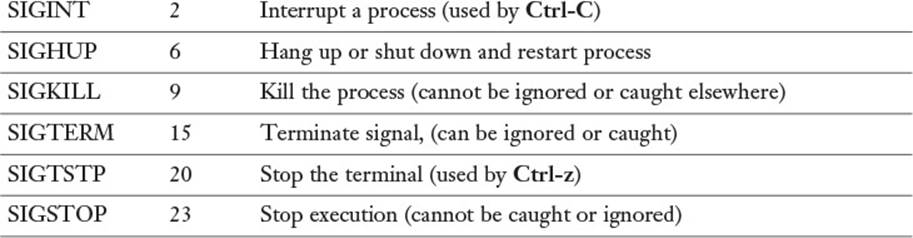
\includegraphics[width=0.8\linewidth]{signals}
\end{center}

\subsection{\texttt{kill}: Inviare segnali ai processi}

Il comando \texttt{kill} può essere utilizzato per inviare un determinato segnale ad un processo.

\begin{code} 
\begin{lstlisting}
# Invia un segnale SIGKILL al processo con PID=150
kill -SIGKILL 150
\end{lstlisting}
\end{code}

\subsection{\texttt{trap}: Intercettare i segnali}

\texttt{trap} è un built-in della shell che permette agli script bash di intercettare dei segnali e di definire degli \textit{handler} personalizzati per gestirli.

La sintassi d'uso è:
\begin{code} 
\begin{lstlisting}
# Esegue il comando echo quando lo script riceve il segnale USR1
trap 'echo ciao' USR1
\end{lstlisting}
\end{code}

Spesso si utilizza una funzione per creare l'handler, segue un esempio:
\begin{code} 
\begin{lstlisting}
#!/bin/bash

# Definisco l'handler personalizzato
function logging () {
	case "$1" in
		start)	echo started  ;;
		stop)	echo stop	  ;;
	esac
}

# Stoppa il logging quando viene ricevuto SIGUSR1
trap 'logging stop' USR1
logging start

while :
do
	# Eseguo le varie elaborazioni
	echo aspetto...
done
\end{lstlisting}
\end{code}



\section{Job control: Inviare processi in background e viceversa}

Da shell può essere molto comodo lanciare dei comandi in background ed eventualmente riportarli in foreground.

\subsection{Avviare un processo in background}

Per avviare un processo in background da shell, basta aggiungere \texttt{\&} al termine del comando:

\begin{code} 
\begin{lstlisting}
# Avvia il comando in background
vim &
\end{lstlisting}
\end{code}

La shell ci restiuisce un \textbf{job id}, che potremo utilizzare successivamente per riportare il processo in foreground.

\begin{info}
	Si può anche portare un processo in background dopo averlo avviato, basta premere \texttt{CTRL+Z} e successivamente digitare \texttt{bg <job\_id>}
	
	\vspace{2mm}
	\textbf{Spiegazione}
	
	Con \texttt{CTRL+Z} si invia al processo un segnale di \texttt{SIGSTOP} che lo blocca. A questo punto, con il comando \texttt{bg} si invia un segnale di \texttt{SIGCONT} che riavvia il processo in background.	
\end{info}

\subsection{Riportare un processo in foreground}

Si può facilmente riportare un processo in foreground con il comando \texttt{fg}.

\begin{code} 
\begin{lstlisting}
# Riporta il processo con il jobid specificato in foreground
fg <job_id>
\end{lstlisting}
\end{code}

\subsection{Visualizzare tutti i jobs attivi}

Per visualizzare l'elenco di tutti i jobs attivi con il loro stato ( attivo o stoppato ), si può utilizzare il comando \texttt{jobs}
\begin{code} 
\begin{lstlisting}
# Elenca tutti i jobs con il loro stato.
jobs
\end{lstlisting}
\end{code}

\section{\texttt{nohup}: Far sopravvivere i processi alla chiusura della shell}

Normalmente, alla chiusura della shell, tutti i processi da lei generati ricevono un segnale di \texttt{SIGHUP} e vengono terminati. Per evitare questo comportamento si può utilizzare il comando \texttt{nohup}, che rende immune il processo all'hangup ed inoltre provvede a scollegare l'output di un processo.

\begin{code} 
\begin{lstlisting}
# Esegue il comando in background e lo
# rende immune alla chiusura della shell
nohup <command> &
\end{lstlisting}
\end{code}

\begin{info}
	A default, \texttt{nohup} ridirige l'output di un processo nel file \texttt{nohup.out}
\end{info}

\section{\texttt{fuser}: Visualizza i processi che usano un file}

\begin{code} 
\begin{lstlisting}
# Visualizza i PID dei processi che usano un file
fuser /path/to/file

# Visualizza i processi che usano un intero filesystem
fuser -m /var
\end{lstlisting}
\end{code}

\subsection{Inviare un segnale a tutti i processi che usano un file}

Tramite l'opzione \texttt{-k} è possibile inviare un segnale a tutti i processi che usano un determinato file:

\begin{code} 
\begin{lstlisting}
# Invia un segnale di SIGUSR1 a tutti i processi che usano il file
fuser -k -USR1 /path/to/file
\end{lstlisting}
\end{code}

\begin{info}
	A causa di una formattazione particolare, analizzare l'output di \texttt{fuser} può essere particolarmente problematico usando \texttt{awk} o \texttt{cut}. In quei casi, conviene usare il comando \texttt{lsof}.
\end{info}

\section{\texttt{lsof}: Lista i file aperti nel sistema}

\texttt{lsof} permette di vedere tutti i file aperti nel sistema.

\begin{code} 
\begin{lstlisting}
# Visualizza tutti i file aperti dal sistema
lsof

# Visualizza i file aperti da uno specifico user
lsof -u <username>

# Visualizza i file aperti da uno specifico processo
lsof -p <PID>

# Limitare l'output di lsof ad una sola directory
lsof +D /path/to/dir

# Listare tutti i file in base al tipo di connessione (tcp o udp)
lsof -i tcp

# IMPORTANTE: Visualizza le porte numeriche e non simboliche
lsof -i tcp -P
\end{lstlisting}
\end{code}

\chapter{Utenti e Gruppi}

\section{\texttt{adduser}: Creare un utente}

Per aggiungere un utente al sistema, si può utilizzare il comando \texttt{adduser}

\begin{code} 
\begin{lstlisting}
# Aggiungi un utente al sistema
adduser <nomeutente>
\end{lstlisting}
\end{code}

\begin{ricordati}
	Per utilizzare \texttt{adduser} sono necessari i permessi di root.
\end{ricordati}

\subsection{Creare un utente con un gruppo specifico}

Normalmente, quando si crea un nuovo utente, questo viene aggiunto ad un nuovo gruppo chiamato come l'utente stesso. Per cambiare questo comportamento, si può utilizzare l'opzione \texttt{--ingroup} di \texttt{adduser}

\begin{code} 
\begin{lstlisting}
# Se non esiste gia', bisogna creare il gruppo
addgroup <nomegruppo>

# A questo punto possiamo creare un nuovo utente ed aggiungerlo al gruppo
adduser --ingroup <nomegruppo> <nomeutente>
\end{lstlisting}
\end{code}

\section{\texttt{addgroup}: Creare un gruppo}

Per creare un nuovo gruppo all'interno del sistema si può utilizzare il comando \texttt{addgroup}
\begin{code} 
\begin{lstlisting}
# Creo un gruppo
addgroup <nomegruppo>
\end{lstlisting}
\end{code}

\section{Aggiungere un utente ad un gruppo}

Per aggiungere un utente ad un gruppo, si può utilizzare il comando \texttt{usermod} in questo modo:
\begin{code} 
\begin{lstlisting}
usermod -a -G <nomegruppo> <nomeutente>
\end{lstlisting}
\end{code}

\begin{info}
	Quando si usa \texttt{usermod} con opzione \texttt{-G}, si aggiunge un gruppo ai \textbf{gruppi secondari} dell'utente. Se si vuole cambiare il \textbf{gruppo primario}, bisogna utilizzare l'opzione \texttt{-g}
	
	\begin{lstlisting}
usermod -g <nomegruppo> <nomeutente>
	\end{lstlisting}
\end{info}

\section{\texttt{id}: Visualizzare le informazioni di un utente}
\label{sec:id}
Si può utilizzare il comando \texttt{id} per ottenere alcune informazioni di un utente, in particolare:
\begin{itemize}
	\item User ID
	\item Group ID
	\item Gruppi secondari
\end{itemize}

\begin{code} 
\begin{lstlisting}
# Visualizzo le info dell'utente corrente
id

# Visualizzo le info di un utente specifico
id <nomeutente>
\end{lstlisting}
\end{code}

\section{Visualizzare i gruppi di cui un utente fa parte}

Per farlo ci sono due modi, il più semplice è utilizzare \texttt{groups}
\begin{code} 
\begin{lstlisting}
# Elenco i gruppi dell'utente corrente
groups

# Elenco i gruppi di un utente specifico
groups <nomeutente>
\end{lstlisting}
\end{code}

In caso si vogliano avere più informazioni ( come i \textbf{group id} ), è possibile utilizzare il comando \texttt{id} ( vedi \ref{sec:id} ).

\section{Vedere tutti i gruppi del sistema}

\begin{code} 
\begin{lstlisting}
# Stampa l'elenco di tutti i gruppi del sistema
getent group
\end{lstlisting}
\end{code}

\section{\texttt{passwd}: Cambiare la password di un utente}

Per cambiare la password di un utente, si può usare il comando \texttt{passwd}

\begin{code} 
\begin{lstlisting}
# Cambia la password dell'utente corrente
passwd

# Cambia la password di un utente specifico
# NOTA: Necessari i permessi di root
passwd <nomeutente>
\end{lstlisting}
\end{code}

\begin{info}
	Utilizzando rispettivamente le opzioni \texttt{-l} e \texttt{-u} è possibile settare un account in stato di lock o unlock. Solo root può farlo.
\end{info}

\section{\texttt{whoami}: Ottieni l'username dell'utente corrente}

Per ottenere l'username dell'utente corrente, si può utilizzare il comando \texttt{whoami}
\begin{code} 
\begin{lstlisting}
# Stampa l'username dell'utente corrente
whoami
\end{lstlisting}
\end{code}

\section{\texttt{who}: Visualizza gli utenti collegati alla macchina}

Serve ad ottenere un elenco degli utenti correntemente collegati alla macchina
\begin{code} 
\begin{lstlisting}
# Elenca gli utenti correntemente collegati alla macchina
who
\end{lstlisting}
\end{code}

\chapter{Permessi}

Su Unix \textbf{tutto è file} ed ognuno di essi è descritto da un identificatore, l'\texttt{i-node}. Tutti sono associati ad un un set di 12 bit che rappresentano i vari permessi.

La seguente figura illustra la disposizione di questi 12 bit:

\begin{center}
	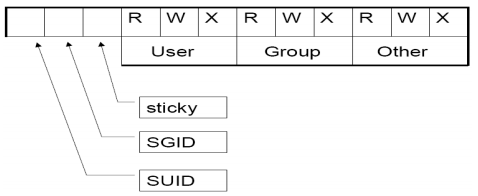
\includegraphics[width=0.6\linewidth]{permessi}
\end{center}

Dove, nel caso di\textbf{ file}:

\begin{itemize}
	\item R = read: Permesso di lettura di un file
	\item W = write: Permesso di scrittura dentro un file
	\item X = execute: Permesso di eseguire il file come programma
\end{itemize}

Mentre, nel caso di una\textbf{ directory}:

\begin{itemize}
	\item R = read: Permesso di elencare i file contenuti al suo interno.
	\item W = write: Permesso di aggiunta/cancellazione/rinomina di un file al suo interno.
	\item X = execute: Permesso di entrare nella directory ( comando \texttt{cd} )
\end{itemize}

\begin{info}
	Il permesso \texttt{write} in una directory permette ad un utente di cancellare qualunque file contenuto in essa, anche se l'utente non ha diritti sul file.
\end{info}

I 3 bit più significativi sono quelli \textbf{speciali} e configurano aspetti particolari:

Nel caso di \textbf{file}:

\begin{itemize}
	\item SUID = Set User ID: In un file eseguibile, se settato a 1, permette di configurare il sistema operativo per \textbf{lanciarlo con l'identità dell'utente proprietario} invece che quella dell'utente che l'ha eseguito.
	
	\item SGID = Set Group ID: Analoga a SUID ma per i gruppi.
	
	\item STICKY BIT: Obsoleto al giorno d'oggi, suggerisce al sistema operativo di tenere una copia del programma in memoria.
\end{itemize}

Nel caso di \textbf{directory}:

\begin{itemize}
	\item SUID = Set User ID: Non viene usato con le directory.
	
	\item SGID = Set Group ID: 
	\begin{itemize}
		\item Precondizioni:
		\begin{itemize}
			\item Un utente appartiene anche al gruppo proprietario della directory
			\item il SGID è settato a 1 sulla directory.
		\end{itemize}
		
		\item Effetto:
		\begin{itemize}
			\item L'utente assume come gruppo attivo il gruppo proprietario della directory
			\item I file creati nella directory hanno quello come gruppo proprietario.
		\end{itemize}
	
		\item Vantaggi ( mantenendo umask 0006 ):
		\begin{itemize}
			\item Nelle aree collaborative i file sono automaticamente resi leggibili e scrivibili da tutti i membri del gruppo
			\item Nelle aree personali i file sono privati perchè di proprietà del gruppo principale dell'utente, che contiene solo l'utente medesimo.
		\end{itemize}
	\end{itemize}
	
	\item STICKY Temp: Se settato a 1 su una directory, impone che i file siano cancellabili solo dal rispettivo proprietario.
\end{itemize}

\section{\texttt{chmod}: Cambiare i permessi di un file}

Per impostare i permessi di un file o di una directory è possibile utilizzare il comando \texttt{chmod}

\begin{code} 
\begin{lstlisting}
# Diamo a tutti il permesso di lettura
chmod a=r <nomefile>

# Aggiungiamo il permesso di scrittura ed esecuzione al proprietario
chmod u+wx <nomefile>

# Rimuoviamo i permessi di scrittura al gruppo proprietario
chmod g-w <nomefile>

# E' anche possibile utilizzare il formato numerico
chmod 0777 <nomefile>
\end{lstlisting}
\end{code}

\section{\texttt{chown}: Cambiare l'ownership di un file}

Per cambiare l'utente o il gruppo proprietario di un file si può utilizzare il comando \texttt{chown}.

\begin{code} 
\begin{lstlisting}
# Cambia l'utente proprietario di un file
chown <username> <nomefile>

# Cambia il gruppo proprietario di un file
# NOTA: Attenzione ad aggiungere :
chown :<group> <nomefile>

# Cambia l'utente ed il gruppo proprietario
chown <username>:<group> <nomefile>

# Cambia la proprieta di tutti i file contenuti nella directory
# in maniera RICORSIVA
chown -R <username>:<group> <nomedirectory>
\end{lstlisting}
\end{code}

\begin{ricordati}
	Per utilizzare con successo il comando \texttt{chown} in generale \textbf{servono i permessi di root}.
\end{ricordati}

\section{\texttt{umask}: Settare i permessi di default}

Per fare in modo che una certa configurazione di permessi venga usata a default per tutti i nuovi file creati, è possibile utilizzare il comando \texttt{umask}. Questo permette di specificare la \textit{maschera} di bit che verrà sottratta ai 12 bit dei permessi.

\begin{center}
	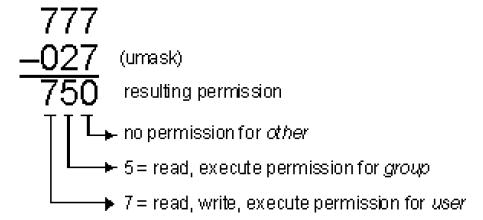
\includegraphics[width=0.5\linewidth]{umask}
\end{center}

\subsection{Visualizzare la maschera corrente}

\begin{code} 
\begin{lstlisting}
# Visualizza la umask corrente
umask

# Per visualizzare i permessi a default correnti in maniera
# piu' comprensibile, si puo' usare l'opzione -S
umask -S
\end{lstlisting}
\end{code}

\subsection{Settare la maschera}

Per settare la maschera, si può utilizzare sempre il comando \texttt{umask}

\begin{code} 
\begin{lstlisting}
# Imposta la maschera in modo che i nuovi file abbiano permesso 775
umask 0002
\end{lstlisting}
\end{code}

\begin{ricordati}
	L'impostazione della \texttt{umask} è valida solo per la sessione di shell corrente. Per fare in modo che l'impostazione sia persistente, bisogna aggiungere il comando \texttt{umask} al file \texttt{/etc/bash.bashrc}
\end{ricordati}

\chapter{Logging}
\label{chap:logging}
Per effettuare logging su linux, si può utilizzare \texttt{rsyslog}. Ogni messaggio di log è caratterizzato dalla coppia:


\begin{center}
	\texttt{<facility>.<priority>}
\end{center}


Dove \texttt{facility} rappresenta l'argomento e può essere:
\begin{multicols}{4}
\begin{itemize}
	\item auth
	\item authpriv
	\item cron
	\item daemon
	\item ftp
	\item kern
	\item lpr
	\item mail
	\item news
	\item syslog
	\item user
	\item uucp
	\item \textbf{local0 .. local7}
\end{itemize}
\end{multicols}

Mentre \texttt{priority} rappresenta la priorità del messaggio e può essere:

\begin{multicols}{4}
	\begin{enumerate}
		\item emerg
		\item alert
		\item crit
		\item err
		\item warning
		\item notice
		\item info
		\item debug
	\end{enumerate}
\end{multicols}

Dove il valore più basso rappresenta la priorità massima. Esempio: \texttt{local0.info}

\section{\texttt{logger}: Loggare un messaggio}
Utilizzando il comando \texttt{logger} è possibile loggare manualmente un messaggio, specificando la \textit{facility} e la \textit{priority}:

\begin{code}
\begin{lstlisting}
# Logga il messaggio "ciao" nella facility local3 con priority info
logger -p local3.info "ciao"
\end{lstlisting}
\end{code}

\section{Impostare la destinazione dei Log}

I vari log possono essere rediretti verso diverse destinazioni. Per farlo, bisogna creare un file \texttt{conf} all'interno della cartella \texttt{/etc/rsyslog.d/}, ad esempio \texttt{/etc/rsyslog.d/lab.conf}

All'interno di questo file è possibile specificare come destinazione dei log sia un file che un server remoto.

\subsection{Salvare i log su file}

E' possibile salvare una certa categoria di log all'interno di un file:

\begin{code}
\begin{lstlisting}
# Salva tutti i log di tipo local0 con qualunque priorita'
local0.*	/var/log/attivita

# Salva i log kernel da livello debug in su
kern.debug	/var/log/attivita

# Salva i log kernel con livello ESATTAMENTE UGUALE a debug
kern.=debug	/var/log/attivita

# NOTA: I due campi sono separati da un TAB
\end{lstlisting}
\end{code}

\begin{ricordati}
	Al termine dell'operazione, riavviare rsyslog con il comando: \texttt{sudo systemctl restart rsyslog}
\end{ricordati}

\begin{ricordati}
	Se elimini direttamente un file di log, potrebbe capitare che il file non venga più ricreato. Per risolvere il problema, puoi riavviare il demone di rsyslog: \texttt{sudo systemctl restart rsyslog}
\end{ricordati}

\subsection{Inviare i log ad un server remoto}

E' possibile inviare una certa categoria di log ad un server remoto, per farlo bisogna impostare correttamente sia il client che il server:

\subsubsection{Configurare il Client}

\begin{code}
\begin{lstlisting}
# Invia all'indirizzo 192.168.56.203 tutti i log di tipo local0 
# con qualunque priorita'
local0.*	@192.168.56.203

# NOTA: I due campi sono separati da un TAB
\end{lstlisting}
\end{code}

\begin{ricordati}
	Al termine dell'operazione, riavviare rsyslog con il comando: \texttt{sudo systemctl restart rsyslog}
\end{ricordati}

\subsubsection{Configurare il Server}

Nel server può essere utile salvare i log ricevuti in un file, come nell'esempio prima:

\begin{code}
\begin{lstlisting}
# Salva tutti i log di tipo local0 con qualunque priorita'
local0.*	/var/log/attivita

# NOTA: I due campi sono separati da un TAB
\end{lstlisting}
\end{code}

Bisogna anche modificare il file \texttt{/etc/rsyslog.conf} per abilitare la ricezione dei log tramite UDP, decommentando:

\begin{code}
\begin{lstlisting}
$ModLoad imudp
$UDPServerRun 514
\end{lstlisting}
\end{code}

\begin{ricordati}
	Al termine dell'operazione, riavviare rsyslog con il comando: \texttt{sudo systemctl restart rsyslog}
\end{ricordati}

\chapter{Cron: Eseguire comandi periodicamente}

Per eseguire dei comandi periodicamente, è possibile utilizzare \textbf{Cron}. Per editare i cronjob da eseguire, si utilizza \texttt{crontab}

È possibile editare il file di configurazione ed aggiungere i vari comandi da eseguire utilizzando il comando:
\begin{code}
\begin{lstlisting}
crontab -e
\end{lstlisting}
\end{code}

Ad ogni comando corrisponde una riga, con il seguente formato:

\begin{center}
	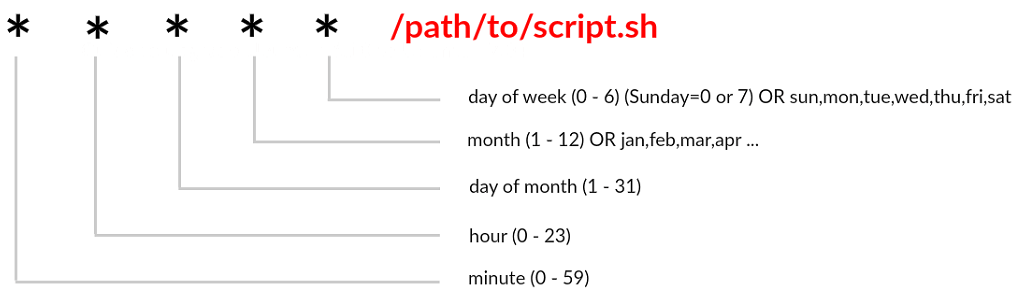
\includegraphics[width=0.8\linewidth]{crontab}
\end{center}

\begin{itemize}
	\item L'\textbf{asterisco (*)} fa match con tutti gli elementi
	\item E' possibile definire un\textbf{ range di valori} con il simbolo \texttt{-}, come ad esempio: \texttt{1-10} oppure \texttt{sun-fri}
	\item E' possibile definire \textbf{multipli range di valori} utilizzando la virgola come separatore: \texttt{jan-mar,jul-sep}
\end{itemize}

\begin{info}
	Di default, usando \texttt{crontab -e} viene editata la configurazione dell'utente corrente. Per \textbf{editare la configurazione di un altro utente} è possibile utilizzare:
	\texttt{crontab -u username -e}
\end{info}

Per listare tutti i cronjob, si può utilizzare il comando:
\begin{code}
\begin{lstlisting}
crontab -l
\end{lstlisting}
\end{code}


\section {Configurazioni di base}

Segue un elenco delle configurazioni di\texttt{ crontab} più comuni:

\subsection{Esegui un job ogni giorno alle 2}
\begin{code}
\begin{lstlisting}
0 2 * * * /bin/sh backup.sh
\end{lstlisting}
\end{code}

\subsection{Esegui un job due volte al giorno}
In questo caso, alle 5 di mattina e alle 5 di pomeriggio.
\begin{code}
\begin{lstlisting}
0 5,17 * * * /scripts/script.sh
\end{lstlisting}
\end{code}

\subsection{Esegui un job ogni minuto}
\begin{code}
	\begin{lstlisting}
* * * * *  /scripts/script.sh
	\end{lstlisting}
\end{code}


\subsection{Esegui un job ogni domenica alle 5}
\begin{code}
	\begin{lstlisting}
0 17 * * sun  /scripts/script.sh
	\end{lstlisting}
\end{code}

\subsection{Esegui un job ogni 10 minuti}
\begin{code}
	\begin{lstlisting}
*/10 * * * * /scripts/monitor.sh
	\end{lstlisting}
\end{code}

\subsection{Esegui un job nei mesi selezionati}
In questo caso a gennaio, maggio ed agosto.
\begin{code}
	\begin{lstlisting}              
* * * jan,may,aug *  /script/script.sh
	\end{lstlisting}
\end{code}

\subsection{Esegui un job nei giorni selezionati}
In questo caso, la domenica ed il venerdi alle 5 di pomeriggio.
\begin{code}
	\begin{lstlisting}              
0 17 * * sun,fri  /script/script.sh
	\end{lstlisting}
\end{code}

\subsection{Esegui un job la prima domenica di ogni mese}
\begin{code}
	\begin{lstlisting}              
0 2 * * sun  [ $(date +%d) -le 07 ] && /script/script.sh
	\end{lstlisting}
\end{code}

\subsection{Esegui un job ogni 4 ore}
\begin{code}
	\begin{lstlisting}              
0 */4 * * * /scripts/script.sh
	\end{lstlisting}
\end{code}

\subsection{Esegui un job due volte ogni domenica e lunedì}
\begin{code}
	\begin{lstlisting}              
0 4,17 * * sun,mon /scripts/script.sh
	\end{lstlisting}
\end{code}

\subsection{Esegui un job ogni 30 secondi}
Eseguire un job con intervalli inferiori al minuto non è possibile nativamente con cron, ma si può usare questo trucco:
\begin{code}
	\begin{lstlisting}              
* * * * * /scripts/script.sh
* * * * *  sleep 30; /scripts/script.sh
	\end{lstlisting}
\end{code}

\subsection{Esegui un più comandi con un solo job}
Con il punto e virgola si possono concatenare più comandi.
\begin{code}
	\begin{lstlisting}              
* * * * * /scripts/script.sh; /scripts/scrit2.sh
	\end{lstlisting}
\end{code}

\subsection{Esegui un job una volta all'anno}
\begin{code}
	\begin{lstlisting}              
@yearly /scripts/script.sh
	\end{lstlisting}
\end{code}

\subsection{Esegui un job una volta al mese}
\begin{code}
	\begin{lstlisting}              
@monthly /scripts/script.sh
	\end{lstlisting}
\end{code}

\subsection{Esegui un job una volta alla settimana}
\begin{code}
	\begin{lstlisting}              
@weekly /bin/script.sh
	\end{lstlisting}
\end{code}

\subsection{Esegui un job ogni giorno}
\begin{code}
	\begin{lstlisting}              
@daily /scripts/script.sh
	\end{lstlisting}
\end{code}

\subsection{Esegui un job ogni ora}
\begin{code}
	\begin{lstlisting}              
@hourly /scripts/script.sh
	\end{lstlisting}
\end{code}

\subsection{Esegui un job al riavvio del sistema}
Questo job verrà eseguito all'avvio del sistema.
\begin{code}
	\begin{lstlisting}              
@reboot /scripts/script.sh
	\end{lstlisting}
\end{code}

\section {Editare crontab da uno script bash}

\subsection{Aggiungere un comando}

La strategia migliore è quella di utilizzare un file temporaneo

\begin{code}
\begin{lstlisting}
# Salva il crontab attuale in un file temporaneo
crontab -l > tmpcron.txt

# Aggiungo il nuovo comando in append al file
echo "* * * * * /bin/echo ciao" >> tmpcron.txt

# Aggiorna il crontab con il nuovo file
crontab tmpcron.txt

# Rimuovo il file temporaneo
rm tmpcron.txt
\end{lstlisting}
\end{code}

\subsection{Rimuovere un comando}

La strategia si avvale di \texttt{grep} per filtrare via la riga da rimuovere.

\begin{code}
\begin{lstlisting}
# Filtro il crontab con grep -v 
# poi lo invio a crontab -
# Che legge da standard input ed aggiorna cron
crontab -l | grep -v "echo ciao" | crontab -
\end{lstlisting}
\end{code}

\section{Correggere il PATH in crontab}

Quando si esegue uno script su crontab, è importante ricordarsi di scrivere i percorsi assoluti dei comandi, perchè cron non ha la conoscenza dei PATH dell'utente.

Un modo per superare questo inconveniente è definire il PATH all'interno del crontab file stesso.
Editando crontab con \texttt{crontab -e} bisogna inserire le due variabili \texttt{SHELL} e \texttt{PATH}.

\begin{code}
\begin{lstlisting}
This has the username field, as used by /etc/crontab.
# /etc/crontab: system-wide crontab
# Unlike any other crontab you don't have to run the `crontab'
# command to install the new version when you edit this file.
# This file also has a username field, that none of the other crontabs do.

SHELL=/bin/sh
PATH=/usr/local/sbin:/usr/local/bin:/sbin:/bin:/usr/sbin:/usr/bin

# m h dom mon dow user   command
42 6 * * *   root    run-parts --report /etc/cron.daily
47 6 * * 7   root    run-parts --report /etc/cron.weekly
52 6 1 * *   root    run-parts --report /etc/cron.monthly
01 01 * * 1-5 root python /path/to/file.py
\end{lstlisting}
\end{code}

\chapter{At: Posticipare l'esecuzione di un comando}

Tramite \texttt{at} è possibile posticipare un comando in modo che venga eseguito successivamente.
La sintassi di base è la seguente: 

\begin{code}
\begin{lstlisting}
# Apre un prompt interattivo per inserire il comando
# da chiudere con Ctrl+D
at <time>

# Da notare che per impostare il comando si puo' usare una pipe
echo 'echo ciao' | at <time>
\end{lstlisting}
\end{code}

Il valore del tempo può assumere diversi valori, seguono alcuni esempi:

\begin{itemize}
	\item \texttt{"9:00 AM"}  : alle 9 di mattina
	\item \texttt{"now + 30 minutes"} : 30 minuti da adesso
	\item \texttt{"now + 30 minutes"} : 30 minuti da adesso
	\item \texttt{"now + 2 days"} : 2 giorni da adesso
\end{itemize}

\section{Visualizzare i task in programma}

Utilizzando il comando \texttt{atq} si possono visualizzare i programmi correntemente in coda.

\begin{info}
	Normalmente \texttt{atq} restituisce i comandi nella coda dell'utente ma, se \textbf{eseguito con permessi di root}, mostra i comandi nelle code di tutti gli utenti.
\end{info}

\section{Rimuovere un lavoro dalla coda}

Utilizzando \texttt{atrm} si può rimuovere un comando dalla coda, la sintassi è la seguente:

\begin{code}
\begin{lstlisting}
# Rimuovo il job con Id 7
atrm 7
\end{lstlisting}
\end{code}

\begin{info}
	Per ottenere l'id del job da eliminare si può utilizzare \texttt{atq} per visionare l'elenco.
\end{info}

\chapter{Configurazioni di Rete}

\section{Verificare che un nodo sia connesso ad un altro}

\subsection{\texttt{ping}}

Il modo più semplice per verificare che un nodo sia connesso ad un altro, e quindi che lo possa raggiungere, è utilizzare il comando \texttt{ping}

Se ad esempio volessimo contattare il server che si trova all'indirizzo \texttt{192.168.56.203}, potremmo, dal client, digitare il comando: \texttt{ping 192.168.56.203}

Se il comando fornisce un output continuo, significa che il nodo è raggiungibile.

\subsection{\texttt{tcpdump}}

Allo stesso modo, nel nodo server, è possibile visualizzare le richieste in arrivo con il comando \texttt{tcpdump}

Individuata l'interfaccia di rete del server, in questo caso \texttt{eth3}, possiamo digitare \texttt{tcpdump -i eth3 -l -n} per visualizzare in tempo reale le richieste \texttt{ICMP} del ping.

\begin{info}
	Per maggiori informazioni su \texttt{tcpdump}, guardare il capitolo \ref{chap:tcpdump}.
\end{info}

\section{Configurazione IP a Runtime}

\subsection{Address}

\begin{code}
\begin{lstlisting}
# Visualizzazione configurazioni IP
ip a

# Assegnazione IP
ip a add <address>/<mask> dev <interface>

# Rimozione IP
ip a del <address>/<mask> dev <interface>
\end{lstlisting}
\end{code}

\subsection {Route}

\begin{code}
\begin{lstlisting}
# Visualizzazione di tutte le Routes
ip r

# Routing via Gateway
ip r add <dst_net>/<mask> via <gw_addr>

# Routing via Interfaccia di rete
ip r add <dst_net>/<mask> dev <interface>

# Rimozione
ip a del <address>/<mask>
\end{lstlisting}
\end{code}

\section{Configurazione IP Permanente}

Bisogna editare il file \texttt{/etc/network/interfaces} ed un tipico esempio è il seguente:

\begin{code}
\begin{lstlisting}
auto eth0                   # Attiva con ifup -a
iface eth0 inet static      # Ip statico definito manualmente
                            # se usate dhcp invece che static,
                            # fa in automatico.
    address 192.168.56.203  
    netmask 255.255.255.0
    gateway 192.168.56.1
    up /path/to/command     # Eseguito dopo la configurazione
\end{lstlisting}
\end{code}

\begin{ricordati}
Dopo la modifica, bisogna riavviare il modulo di networking.
\begin{lstlisting}
sudo systemctl stop networking
sudo systemctl start networking
\end{lstlisting}

Se qualche interfaccia non riparte, usare:
\begin{lstlisting}
ifup <nome_interfaccia>
\end{lstlisting}

Se, dopo averle rimosse, restano delle interfacce ancora attive, utilizzare:
\begin{lstlisting}
ip addr del <indirizzo>/<mask> dev <nome_interfaccia>
\end{lstlisting}
\end{ricordati}

\section{Configurazione IP Forwarding}

E' possibile configurare l'IP forwarding in maniera tale che il \textbf{client} possa comunicare con il \textbf{server} tramite il \textbf{router}, come in figura \ref{fig:forwarding}.

\begin{figure}
	\centering
	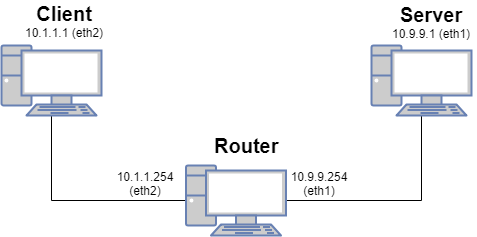
\includegraphics[width=0.7\linewidth]{forwarding}
	\caption{Architettura forwarding}
	\label{fig:forwarding}
\end{figure}

Per farlo, è necessario configurare le tre macchine come segue:

\subsection{Client}

Editando il file \texttt{/etc/network/interfaces}

\begin{code}
\begin{lstlisting}
auto eth2
iface eth2 inet static
	address 10.1.1.1
	netmask 255.255.255.0
	up ip route add 10.9.9.0/24 via 10.1.1.254
\end{lstlisting}
\end{code}

\begin{ricordati}
Dopo la modifica, bisogna riavviare il modulo di networking.
\begin{lstlisting}
sudo systemctl stop networking
sudo systemctl start networking
\end{lstlisting}

Se qualche interfaccia non riparte, usare:
\begin{lstlisting}
ifup <nome_interfaccia>
\end{lstlisting}

Se, dopo averle rimosse, restano delle interfacce ancora attive, utilizzare:
\begin{lstlisting}
ip addr del <indirizzo>/<mask> dev <nome_interfaccia>
\end{lstlisting}
\end{ricordati}

\subsection{Router}

Editando il file \texttt{/etc/network/interfaces}

\begin{code}
\begin{lstlisting}
auto eth1
iface eth1 inet static
	address 10.9.9.254
	netmask 255.255.255.0

auto eth2
iface eth2 inet static
	address 10.1.1.254
	netmask 255.255.255.0
\end{lstlisting}
\end{code}

\begin{ricordati}
	Dopo la modifica, bisogna riavviare il modulo di networking.
\begin{lstlisting}
sudo systemctl stop networking
sudo systemctl start networking
\end{lstlisting}

Se qualche interfaccia non riparte, usare:
\begin{lstlisting}
ifup <nome_interfaccia>
\end{lstlisting}

Se, dopo averle rimosse, restano delle interfacce ancora attive, utilizzare:
\begin{lstlisting}
ip addr del <indirizzo>/<mask> dev <nome_interfaccia>
\end{lstlisting}
\end{ricordati}

Bisogna abilitare il forwarding, editando il file \texttt{/etc/sysctl.conf} ed assicurandosi che sia presente, non commentato, questo comando:

\begin{code}
\begin{lstlisting}
net.ipv4.ip_forward=1
\end{lstlisting}
\end{code}

\begin{ricordati}
	Dopo la modifica, bisogna lanciare:
\begin{lstlisting}
sudo sysctl -p
\end{lstlisting}
\end{ricordati}

\subsection{Server}

Editando il file \texttt{/etc/network/interfaces}

\begin{code}
\begin{lstlisting}
auto eth1
iface eth1 inet static
	address 10.9.9.1
	netmask 255.255.255.0
	up ip route add 10.1.1.0/24 via 10.9.9.254
\end{lstlisting}
\end{code}

\begin{ricordati}
Dopo la modifica, bisogna riavviare il modulo di networking.
\begin{lstlisting}
sudo systemctl stop networking
sudo systemctl start networking
\end{lstlisting}

Se qualche interfaccia non riparte, usare:
\begin{lstlisting}
ifup <nome_interfaccia>
\end{lstlisting}

Se, dopo averle rimosse, restano delle interfacce ancora attive, utilizzare:
\begin{lstlisting}
ip addr del <indirizzo>/<mask> dev <nome_interfaccia>
\end{lstlisting}
\end{ricordati}

\section{\texttt{ss}: Ottenere informazioni sulle socket}

\texttt{ss} è un comodo strumento che permette di ottenere delle informazioni riguardo all'utilizzo di socket nel sistem:

 \begin{code}
\begin{lstlisting}
# Visualizza le connessioni tcp nel sistema, visualizzando anche
# i processi e gli utenti coinvolti
ss -tpn

# Con l'udp invece
ss -upn
\end{lstlisting}
 \end{code}

\chapter{\texttt{ssh}: Secure Shell}

Il comando \texttt{ssh} permette di ottenere il terminale di una macchina remota.

\section{Eseguire remotamente un comando}

Oltre a poter aprire una shell interattiva, \texttt{ssh} permette anche di inviare singoli comandi alla macchina remota:
\begin{code}
\begin{lstlisting}
# Eseguo il comando ls sulla macchina remota
ssh las@192.168.56.201 ls
\end{lstlisting}
\end{code}

\section{Variabili d'ambiente SSH}

All'interno di una shell \texttt{ssh} sono presenti alcune variabili di sistema che permettono di ottenere delle informazioni riguardo alla connessione corrente:

\begin{code}
\begin{lstlisting}
# Ad esempio
SSH_CLIENT='192.168.56.1 56156 22'
SSH_CONNECTION='192.168.56.1 56156 192.168.56.201 22'
SSH_TTY=/dev/pts/0
\end{lstlisting}
\end{code}

\section{Configurare il login tramite chiave pubblica}

Configurando l'accesso con chiave pubblica permette di effettuare il login con \texttt{ssh} senza digitare la password.

\subsection{Configurare la macchina HOST}
Sulla macchina HOST dovremo generare una coppia di chiavi (pubblica + privata) e poi inviare la propria chiave pubblica alla macchina remota.

\begin{code}
\begin{lstlisting}
# Genero la coppia di chiavi
# NOTA: premere invio ad ogni domanda
ssh-keygen -t rsa -b 2048

# Invio alla macchina remota la chiave pubblica
# NOTA: Cambiare l'indirizzo di destinazione all'occorrenza
scp .ssh/id_rsa.pub las@192.168.56.201:
\end{lstlisting}
\end{code}

\begin{ricordati}
	Per eseguire correttamente il login remoto, assicurati di avere nella cartella \texttt{.ssh} il file "\texttt{id\_rsa}".
	Questo viene automaticamente generato da \texttt{ssk-keygen} e rappresenta la tua chiave privata.
\end{ricordati}

\begin{info}
	In caso sia necessario utilizzare una chiave diversa da quella di default: \texttt{id\_rsa} è possibile utilizzare l'opzione \texttt{-i} e specificare un file per la chiave privata.
\end{info}

\subsection{Configurare la macchina REMOTA}
Una volta ricevuta la chiave pubblica, bisogna aggiungerla all'elenco delle chiavi autorizzate:

\begin{code}
\begin{lstlisting}
# Se non esiste, creo la cartella .ssh con i giusti permessi
mkdir .ssh
chmod 700 .ssh

# Aggiungo alla coda del file .ssh/authorized_keys la chiave
cat id_rsa.pub >> .ssh/authorized_keys
\end{lstlisting}
\end{code}

\chapter{\texttt{iptables}: Stateful packet filtering}

%TODO Aggiungere funzioni utili di iptables

\texttt{IPTABLES} implementa la funzionalità di stateful packet filtering a livello di kernel ed ha il controllo dei pacchetti in transito sulle interfacce di rete.
I pacchetti sono sottoposti a diverse modalità di elaborazione chiamate \textbf{table}, ciascuna delle quali composta da gruppi di regole chiamate \textbf{chain}.

\begin{figure}[!htb]
	\centering
    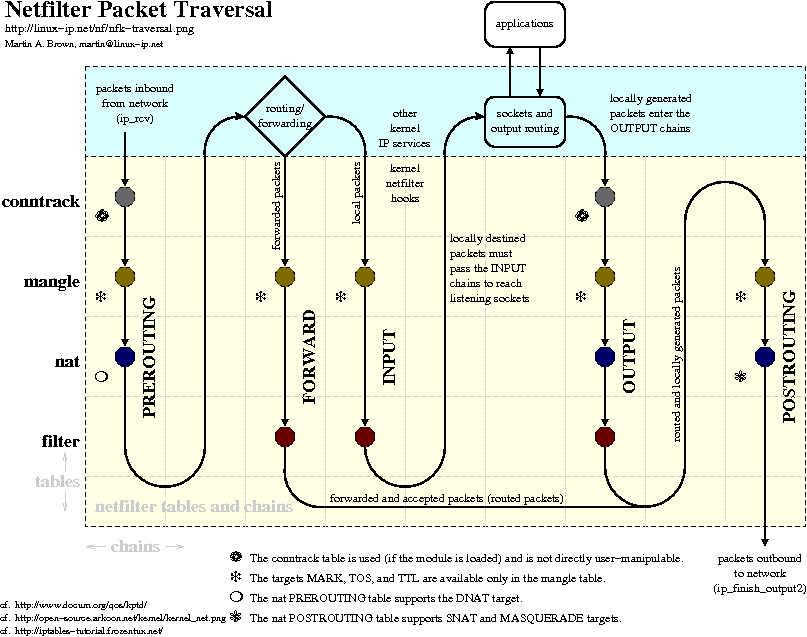
\includegraphics[width=\linewidth]{iptables}
    \caption{Schema architetturale delle IPTABLES}
\end{figure}

\section{Tabella \texttt{FILTER}: Funzionalità di firewall}

La tabella di \texttt{FILTER} permette di definire le regole di firewall vere e proprie. Al suo interno sono contenute tre \textbf{chain} predefinite:

\begin{itemize}
	\item \texttt{INPUT}: contiene le regole di filtraggio da applicare ai pacchetti in arrivo.
	\item \texttt{OUTPUT}: contiene le regole di filtraggio da applicare ai pacchetti in uscita
	\item \texttt{FORWARD}: contiene le regole di filtraggio da applicare ai pacchetti in transito per il firewall ( inoltrate da interfacce diverse )
\end{itemize}

\subsection{Visualizzare le regole attuali}

\begin{code}
\begin{lstlisting}
# Visualizza le configurazioni di iptables
iptables -vnxL --line-numbers
\end{lstlisting}
\end{code}

\begin{ricordati}
	Per utilizzare il comando \texttt{iptables} bisogna avere permessi di \textbf{root}.
\end{ricordati}

\subsection{Aggiungere nuove regole}

L'amministratore può personalizzare il comportamento del firewall aggiungendo nuove regole che, alla fine dell'elaborazione, dovranno stabilire uno dei tre possibili esiti:

\begin{itemize}
	\item \texttt{DROP}: Scarta il pacchetto
	\item \texttt{REJECT}: Scarta il pacchetto ed invia un pacchetto \texttt{ICMP} per segnalare l'errore al mittente.
	\item \texttt{ACCEPT}: Accetta il pacchetto.
\end{itemize}

Una regola può essere aggiunta sia \textbf{in testa} che \textbf{in coda} alle regole già presenti nella chain:

\begin{code}
\begin{lstlisting}
# Aggiungo una regola in coda ( APPEND ) alla chain FORWARD
iptables -A FORWARD <options> -j ACCEPT

# Aggiungo una regola all'inizio della coda ( INSERT )
iptables -I FORWARD <options> -j ACCEPT
\end{lstlisting}
\end{code}

Si possono specificare un gran numero di opzioni per migliorare il filtraggio dei pacchetti, le più importanti sono:

\begin{code}
\begin{lstlisting}
-i eth3       # Solo pacchetti in ingresso dall'interfaccia eth3
-o eth3       # Solo pacchetti in uscita dall'interfaccia eth3
-s <ip>       # Pacchetti che provengono dall'ip specificato
-d <ip>       # Pacchetti destinati all'ip specificato
-p tcp        # Solo pacchetti TCP
# Specificando il protocollo tcp o udp, si possono selezionare le porte:
--dport <prt> # Pacchetti con porta di destinazione == <prt>
--sport <prt> # Pacchetti con porta di partenza == <prt>
# Nel caso del protocollo TCP, anche lo stato della connessione:
-m state --state NEW,ESTABLISHED
\end{lstlisting}
\end{code}

\begin{ricordati}
	Se un pacchetto non soddisfa nessuna regola, \textbf{viene applicata la \textit{policy} di default}.
\end{ricordati}

\begin{ricordati}
	Le regole \texttt{iptables} vengono resettate allo spegnimento della macchina, se si vogliono rendere persistenti è quindi importante aggiungerle al file \texttt{.bashrc}
\end{ricordati}

\subsection{Abilitare LOOPBACK e SSH}

Alcune regole sono molto importanti e vanno sempre specificate prima di introdurre delle nuove policy di default.

\begin{code}
\begin{lstlisting}
# Accetta tutti i pacchetti dell'interfaccia di loopback
iptables -I INPUT -i lo -s 127.0.0.0/8 -j ACCEPT
iptables -I OUTPUT -o lo -d 127.0.0.0/8 -j ACCEPT

# Consenti le connessioni SSH ( in questo caso verso router )
iptables -I INPUT -i eth3 -s 192.168.56.1 -d 192.168.56.202 \
         -p tcp --dport 22 -j ACCEPT
iptables -I OUTPUT -o eth3 -d 192.168.56.1 -s 192.168.56.202 \
         -p tcp --sport 22 -m state --state ESTABLISHED -j ACCEPT
\end{lstlisting}
\end{code}

\subsection{Eliminare una regola}

Per eliminare una regola, si può far uso dell'opzione \texttt{-D}, specificando il numero di regola oppure riportando la regola per intero.

\begin{code}
\begin{lstlisting}
# Elimina la regola numero 2 della chain INPUT
iptables -D INPUT 2

# Se ad esempio aggiungiamo una regola del tipo
iptables -A INPUT -s 10.1.1.1 -j ACCEPT
# Possiamo eliminarla con
iptables -D INPUT -s 10.1.1.1 -j ACCEPT

# E' inoltre possibile eleminare tutte le regole
# di una chain ( FLUSH )
iptables -F INPUT
\end{lstlisting}
\end{code}

\begin{pattern}
Spesso è comodo definire una funzione per aggiungere un set di regole a \texttt{iptables} \textbf{parametrizzando} il tipo di operazione. Questo permette di aggiungere e rimuovere queste regole con facilità.

\begin{lstlisting}
# ARGOMENTI: $1 A oppure D per aggiungere o togliere la regola.
function gestisciRegola () {
	iptables -$1 INPUT -s 10.1.1.1 -j ACCEPT
}

# Esempio d'uso
gestisciRegola A   # Aggiungo la regola
gestisciRegola D   # Elimino la regola
\end{lstlisting}
\end{pattern}

\subsection{Impostare le policy di default}

Per impostare la policy di default, si può utilizzare l'opzione \texttt{-P}
\begin{code}
\begin{lstlisting}
# Imposto tutte le policy di default droppando i pacchetti che non 
# soddisfano le regole
iptables -P INPUT DROP
iptables -P OUTPUT DROP
iptables -P FORWARD DROP
\end{lstlisting}
\end{code}

\begin{ricordati}
	Quando vengono definite le policy di default a \texttt{DROP} è molto importante aggiungere delle regole per l'interfaccia di loopback e per la connessione ssh, altrimenti il sistema potrebbe non funzionare correttamente.
\end{ricordati}

\subsection{Loggare pacchetti con \texttt{iptables}}

Definendo come policy \texttt{LOG} è possibile loggare i pacchetti in transito:

\begin{code}
\begin{lstlisting}
# Inserisce una regola che logga i pacchetti in transito nella chain
# specificata con prefisso e livello di log specificati
iptables -I <chain> <options> -j LOG --log-prefix=" prefisso " \
         --log-level <livello_log>
\end{lstlisting}
\end{code}

\begin{info}
	I log hanno \textit{facility} = \texttt{kernel}, questo implica che se ad esempio specifichiamo \texttt{log-level=debug}, i log verranno salvati con livello \texttt{kernel.debug}
	
	E' possibile specificare un file di destinazione apposito, per ulteriori informazioni guardare il capitolo \ref{chap:logging}.
\end{info}

\subsection{Rilevare inizio e fine di una connessione TCP}

Un caso di notevole interesse è la rilevazione dell'inizio e la fine di una connessione tcp. Nell'esempio sottostante, vengono loggati l'evento di fine ed inizio.

\begin{code}
\begin{lstlisting}
# Logga l'inizio di ogni connessione inoltrata da 10.1.1.1 a 10.9.9.1
# con livello debug e prefisso NEWCON
iptables -I FORWARD -i eth2 -s 10.1.1.1 -d 10.9.9.1 -p tcp \
 --tcp-flags SYN SYN -j LOG --log-prefix " NEWCON " --log-level debug
 
# Logga la fine di ogni connessione inoltrata da 10.1.1.1 a 10.9.9.1
# con livello debug e prefisso ENDCON
iptables -I FORWARD -i eth2 -s 10.1.1.1 -d 10.9.9.1 -p tcp \
 --tcp-flags FIN FIN -j LOG --log-prefix " ENDCON " --log-level debug
\end{lstlisting}
\end{code}

\section{Tabella \texttt{NAT}: Effettuare il NAT sui pacchetti in transito}

La tabella \texttt{NAT} permette di effettuare delle modifiche ai pacchetti in modo che risultino traslate a livello di indirizzo.
Lavora sui pacchetti \textit{forwarded}, questo implica che \textbf{per utilizzare il \texttt{NAT} è necessario abilitare le regole di \texttt{FORWARD}} esposte in precedenza.

\subsection{Destination NAT}

Il \textit{Destination NAT} permette di intercettare le connessioni da Client a Router, ridirigendole automaticamente al Server. In pratica Router \textit{impersona} Server ed il Client non si accorge di nulla.

\begin{figure}[htb!]
	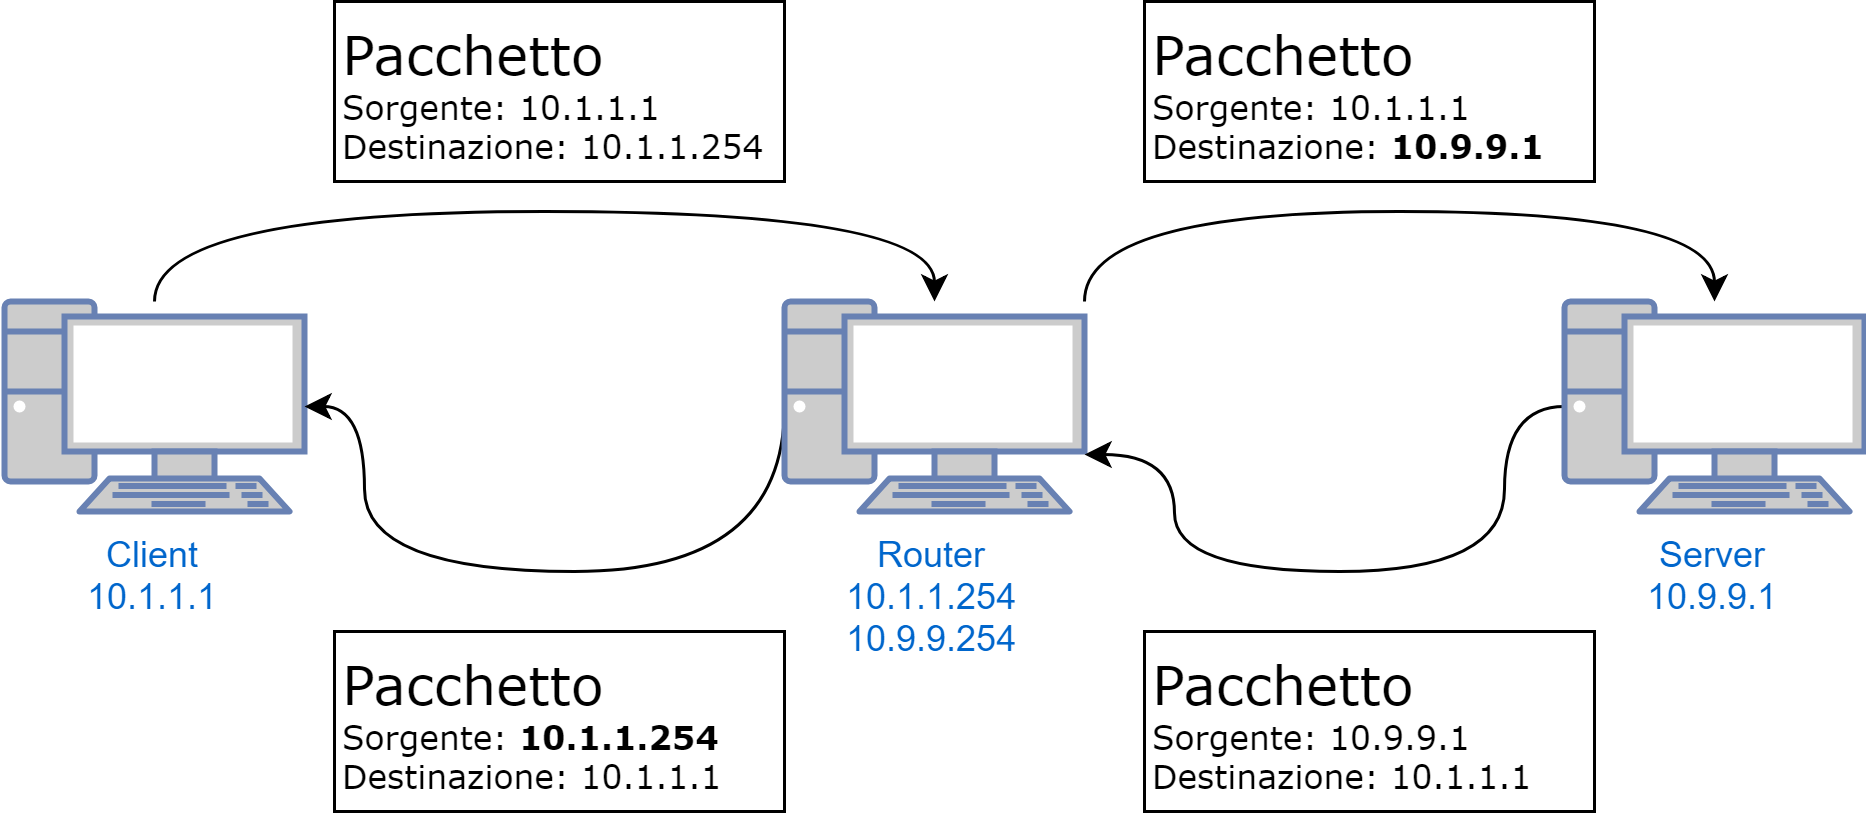
\includegraphics[width=\linewidth]{DNAT}
	\caption{Esempio di Destination NAT. In grassetto gli indirizzi modificati.}
\end{figure}

\begin{code}
\begin{lstlisting}
# Intercetta le connessioni SSH da Client a Router e le ridirige a Server
iptables -t nat -A PREROUTING -i eth2 -s 10.1.1.1 -d 10.1.1.254 \
         -p tcp --dport 22 -j DNAT --to-dest 10.9.9.1
\end{lstlisting}
\end{code}

\begin{ricordati}
	Ricordati di impostare le regole di \texttt{FORWARD} di \texttt{iptables} in modo che i pacchetti possano essere inoltrati da Router, altrimenti il \texttt{NAT} non funzionerà. Per testare la configurazione iniziale, puoi impostare momentaneamente le policy di \texttt{FORWARD} come \texttt{ACCEPT}
	\begin{lstlisting}
iptables -P FORWARD ACCEPT
	\end{lstlisting}
\end{ricordati}


\subsection{Source NAT}

Il \textit{Source NAT} permette di mascherare la sorgente di un pacchetto, in modo che \textbf{la destinazione} non veda il mittente originale. In pratica, quanto il Client invia un pacchetto al Server, questo lo riceve come se \textbf{lo avesse mandato il Router}. Quando poi il Server invierà la risposta al Router, questo si occuperà di inoltrarla al Client.

\begin{figure}[htb!]
	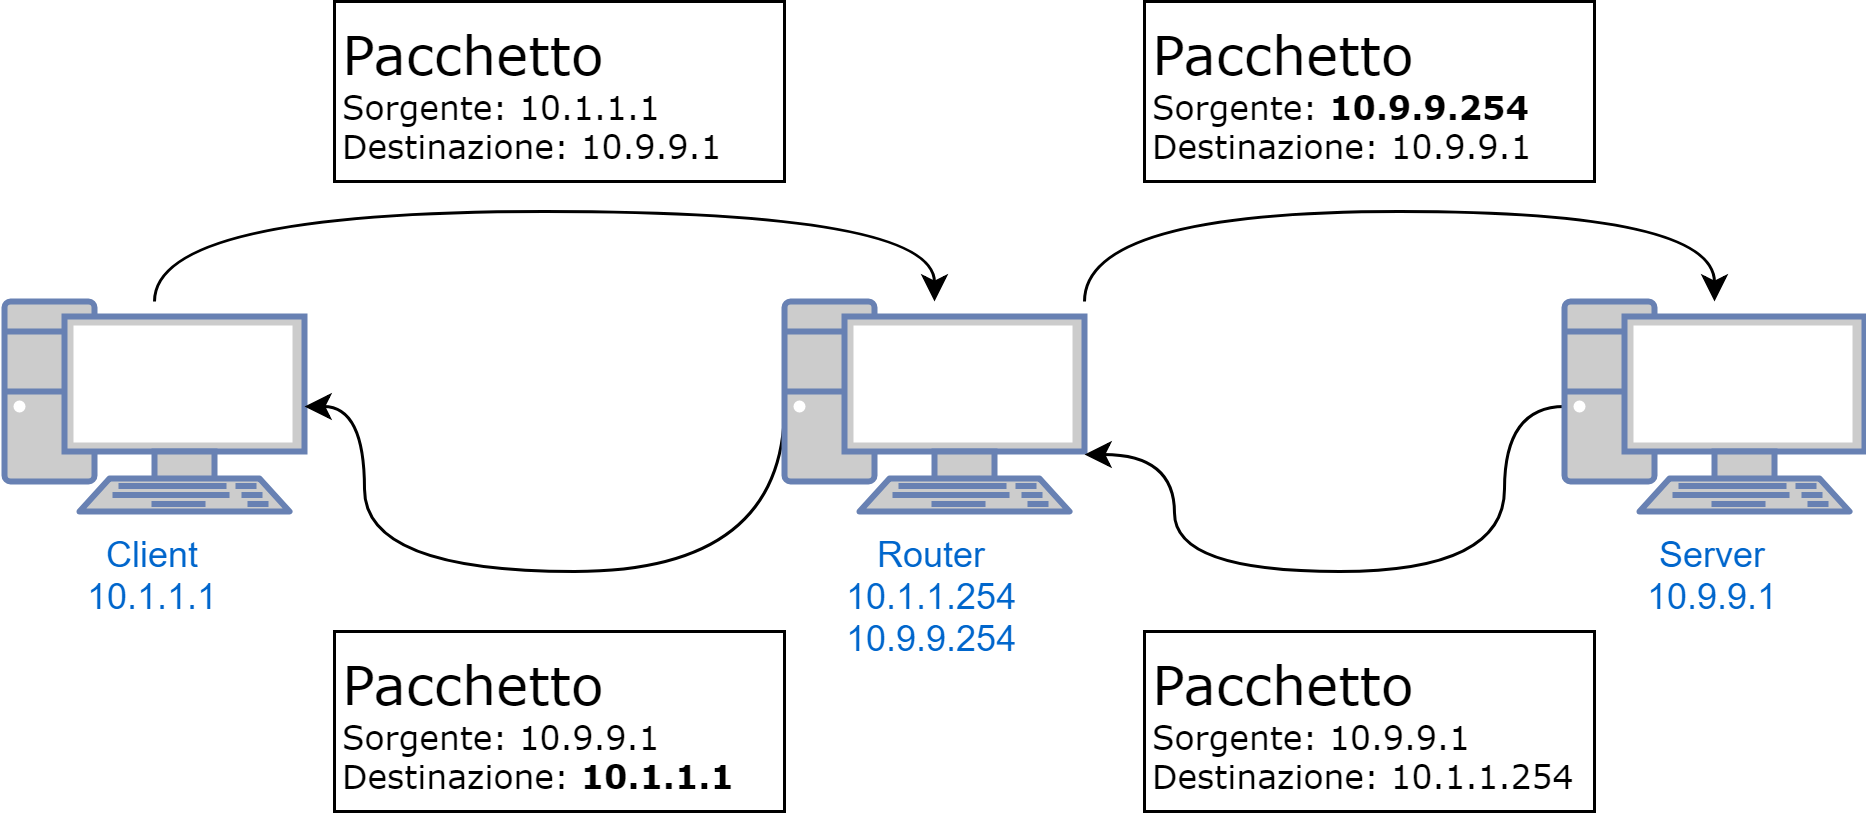
\includegraphics[width=\linewidth]{SNAT}
	\caption{Esempio di Source NAT. In grassetto gli indirizzi modificati.}
\end{figure}

\begin{code}
\begin{lstlisting}
# Espone le connessioni dal Client al Server come se venissero 
# da Router stesso
iptables -t nat -A POSTROUTING -o eth1 -s 10.1.1.1 -d 10.9.9.1 \
         -j SNAT --to-source 10.9.9.254
\end{lstlisting}
\end{code}

\begin{ricordati}
	Ricordati di impostare le regole di \texttt{FORWARD} di \texttt{iptables} in modo che i pacchetti possano essere inoltrati da Router, altrimenti il \texttt{NAT} non funzionerà. Per testare la configurazione iniziale, puoi impostare momentaneamente le policy di \texttt{FORWARD} come \texttt{ACCEPT}
	\begin{lstlisting}
iptables -P FORWARD ACCEPT
	\end{lstlisting}
\end{ricordati}

\section{Chain personalizzate}

Con \texttt{iptables} è possibile creare delle chain personalizzate:

\begin{code}
\begin{lstlisting}
# Crea la chain PIPPO
iptables -N PIPPO

# Inserisco una regola all'interno di PIPPO che faccia direttamente il
# RETURN ( ovvero ritorni alla chain che l'ha invocata )
iptables -I PIPPO -j RETURN

# Elimino tutte le regole all'interno di PIPPO ( FLUSH )
iptables -F PIPPO

# Elimino la chain PIPPO
iptables -X PIPPO
\end{lstlisting}
\end{code}

\section{Salvare e ripristinare le regole di \texttt{iptables}}

Le regole di \texttt{iptables} vengono perse ad ogni riavvio della macchina. Per renderle persistenti è quindi necessario ricaricarle ad ogni avvio. Gli strumenti \texttt{iptables-save} e \texttt{iptables-restore} permettono di salvare e in seguito ripristinare la configurazione corrente.

\begin{code}
\begin{lstlisting}
# Salva la configurazione corrente sul file
iptables-save > output.txt

# Ripristina la configurazione salvata
iptables-restore < output.txt
\end{lstlisting}
\end{code}
	
\chapter{tcpdump: Sniffing dei pacchetti}
\label{chap:tcpdump}

\texttt{tcpdump} è uno strumento che permette di intercettare e leggere i pacchetti TCP/IP in transito.

\section{Principali opzioni}
\begin{code}
\begin{lstlisting}
-i any       # Ascolta da tutte le interfacce di rete
-i eth0      # Ascolta sull'interfaccia eth0
-l           # IMPORTANTE Line-buffered: Stampa un pacchetto appena 
             # lo riceve senza bufferizzare. 
-n           # IMPORTANTE Non risolvere gli hostname, lascia numerico
-t           # Stampa il tempo in un formato human-friendly
-c [N]       # Legge solo N pacchetti e poi termina
-w output    # Scrive i pacchetti nel file PCAP di output
-r file      # Legge i pacchetti dal file PCAP
-p           # No promiscuous mode
-A           # Stampa i pacchetti in ASCII
-X           # Stampa i pacchetti in ASCII ed esadecimale
\end{lstlisting}
\end{code}

\begin{ricordati}
	Per rilevare in real-time i pacchetti è molto importante specificare le opzioni \texttt{-l} e \texttt{-n} che permettono rispettivamente di non bufferizzare e di evitare di risolvere gli hostname.
\end{ricordati}

\section{Filtrare i pacchetti}

\texttt{tcpdump} offre una grande quantità di filtri per scremare i pacchetti.

\begin{info}
	Per leggere tutte le informazioni sui filtri di \texttt{tcpdump}, guardare la man page relativa ai \texttt{pcap-filter}
\end{info}

\subsection{Filtrare i pacchetti in base alla destinazione o alla sorgente}

\begin{code}
\begin{lstlisting}
# Leggi i pacchetti in arrivo da 10.9.9.1
tcpdump src 10.9.9.1

# Leggi i pacchetti destinati a 10.9.9.1
tcpdump dst 10.9.9.1
\end{lstlisting}
\end{code}

\subsection{Filtra i pacchetti in base al network}

\begin{code}
\begin{lstlisting}
# Leggi i pacchetti relativi al network 10.9.9.0/24
tcpdump net 10.9.9.0/24
\end{lstlisting}
\end{code}

\subsection{Filtra il traffico legato ad una porta}
\begin{code}
\begin{lstlisting}
# Leggi i pacchetti relativi alla porta 1234
tcpdump port 1234

# Leggi i pacchetti in arrivo dalla porta 1234
tcpdump src port 1234
\end{lstlisting}
\end{code}

\subsection{Filtra il traffico legato ad un protocollo}
\begin{code}
\begin{lstlisting}
# Leggi i pacchetti relativi al protocollo icmp
tcpdump icmp

# Leggi i pacchetti relativi a udp
tcpdump udp
\end{lstlisting}
\end{code}

\subsection{Filtra il traffico in base alla dimensione del pacchetto}
\begin{code}
\begin{lstlisting}
# Leggi i pacchetti con dimensione minore di 32 byte
tcpdump less 32

# Leggi i pacchetti con dimensione maggiore di 32 byte
tcpdump greater 32

# Si possono concatenare
tcpdump less 32 and greater 20
\end{lstlisting}
\end{code}

\section{Combinare i filtri}

Per combinare i filtri si possono utilizzare \texttt{and}, \texttt{or} e \texttt{not}.
\begin{code}
\begin{lstlisting}
# Traffico destinato a 192.168.0.2 e non di tipo icmp
tcpdump dst 192.168.0.2 and not icmp

# Traffico da un host ma non su una specifica porta
# Utile per filtrare connessione SSH
tcpdump src 10.9.9.1 and not dst port 22

# Con le parentesi si possono anche creare regole piu complesse
tcpdump src 10.9.9.1 and (dst port 1234 or 22)
\end{lstlisting}
\end{code}

\section{Catturare i pacchetti con flag TCP particolari}
\begin{code}
\begin{lstlisting}
# Cattura i pacchetti con dei flag tcp settati:

tcpdump 'tcp[tcpflags] == tcp-syn'
tcpdump 'tcp[tcpflags] == tcp-fin'
\end{lstlisting}
\end{code}

\chapter{\texttt{SNMP}: Simple Network Management Protocol}

Il protocollo \texttt{SNMP} permette di gestire in maniera semplificata diverse risorse di rete. Ogni oggetto è rappresentato da un \textit{OID} univoco ed incluso in un database detto \textit{MIB}.

\section{Configurare il demone SNMPD}

Prima di poter eseguire delle richieste è necessario impostare il demone snmp del server. In particolare:

\begin{code}
\begin{lstlisting}
# Nel file: /etc/snmp/snmp.conf
# Commentare la riga "mibs :" per avere i nomi simbolici
\end{lstlisting}
\end{code}

\begin{code}
\begin{lstlisting}
# Nel file: /etc/snmp/snmpd.conf
# Sistituire
agentAddress udp:127.0.0.1:161
# con
agentAddress udp:161

# Definire una vista che includa tutto il MIB
view	all	included 	.1

# Abilitare le community ad operare su quella vista
rocommunity public default -V all
rwcommunity supercom default -V all
\end{lstlisting}
\end{code}

\begin{ricordati}
	Dopo ogni cambio di configurazione, bisogna riavviare il demone SNMP tramite il comando:
	\begin{lstlisting}
sudo systemctl restart snmpd
	\end{lstlisting}
\end{ricordati}

\section{Visualizzare tutte le entry}

Per visualizzare tutti gli oggetti di un server, si può utilizzare il comando \texttt{snmpwalk}:

\begin{code}
\begin{lstlisting}
# Visualizza tutti gli oggetti del server 10.9.9.1
snmpwalk -v 1 -c public 10.9.9.1 .1

# Pue' essere utile utilizzare in piping il comando less
snmpwalk -v 1 -c public 10.9.9.1 .1 | less
\end{lstlisting}
\end{code}

\section{Ottenere il valore di una entry}

\begin{code}
\begin{lstlisting}
# Visualizza il valore di una specifica entry
snmpget -v 1 -c public 192.168.56.203 'UCD-SNMP-MIB:memAvailReal.0'
\end{lstlisting}
\end{code}

\section{Estendere le funzionalità di SNMP}

È possibile estendere le funzionalità di SNMP aggiungendo delle direttive \texttt{extend} nel file di configurazione \texttt{/etc/snmp/snmpd.conf}

\begin{code}
\begin{lstlisting}
# Da aggiungere al file /etc/snmp/snmpd.conf

# Restituisce la data corrente
extend currdate /bin/date

# Restituisce il numero di processi in esecuzione sulla macchina
extend-sh sshnum ps haux | wc -l
\end{lstlisting}
\end{code}

\begin{info}
	Utilizzando la direttiva \texttt{extend-sh} è possibile invocare direttamente dei comandi di shell.
\end{info}

\begin{ricordati}
	Per vedere gli effetti della modifica al file di configurazione, bisogna riavviare il demone SNMP tramite: 
	
	\begin{lstlisting}
sudo systemctl restart snmpd
	\end{lstlisting}
\end{ricordati}

\begin{ricordati}
	I valori definiti tramite \texttt{extend} non sono aggiornati ad ogni richiesta, ma vengono salvati in \textbf{cache}, generalmente aggiornata ogni 5 secondi.
\end{ricordati}

\subsection{Leggere il valore di un campo personalizzato}

Per ottenere il valore di un campo creato tramite \texttt{extend}, si può utilizzare:
\begin{code}
\begin{lstlisting}
# Legge il valore di "sshnum" definito precedentemente
snmpget -v 1 -c public <indirizzo_macchina> \
 'NET-SNMP-EXTEND-MIB::nsExtendOutputFull."sshnum"'

# Per ottenere il valore puro si puo' utilizzare AWK
snmpget -v 1 -c public <indirizzo_macchina> \
 'NET-SNMP-EXTEND-MIB::nsExtendOutputFull."sshnum"' | \
awk -F 'STRING: ' '{ print $2 }' 
\end{lstlisting}
\end{code}

\subsection{Estendere la funzionalità con un comando root}

Per fare in modo che SNMP possa essere esteso per eseguire un comando di root sono necessari alcuni passaggi:

\begin{enumerate}
	\item Editare il file di configurazione \texttt{/etc/snmp/snmpd.conf} per includere la nuova regola:
	\begin{code}
\begin{lstlisting}
# NOTARE la presenza di /usr/bin/sudo
# Restituisce le connessioni correntemente attive
extend    activeconn /usr/bin/sudo /bin/ss -ntp
\end{lstlisting}
	\end{code}
	\item Aggiungere una regola in \texttt{/etc/sudoers} ( tramite il comando \texttt{sudo visudo} ) per permettere al demone \texttt{snmp} di eseguire il comando come \textbf{root}:
		\begin{code}
\begin{lstlisting}
# NOTA: Per editare il file conviene usare: sudo visudo
# Permette all'utente snmp di eseguire il comando ss
# senza digitare la password
snmp	ALL=NOPASSWD:/bin/ss
\end{lstlisting}
	\end{code}
\end{enumerate}

\begin{info}
	Si può testare l'esito di questa operazione impersonando l'utente \texttt{snmp} e cercando di eseguire il comando che richiede permessi di \textbf{root}. Per farlo bisogna diventare root ( usando il comando \texttt{sudo -i} ) e successivamente aprire una shell come utente \texttt{snmp}:
	
	\begin{lstlisting}
# Apre una shell come utente snmp
# NOTA: Bisogna essere root per riuscirci
su -s /bin/bash - snmp
	\end{lstlisting}
\end{info}

\section{Ottenere informazioni riguardo un processo}

\texttt{SNMP} può essere configurato per monitorare un processo in esecuzione e fornire diversi parametri a riguardo.

Il primo passo è modificare il file di configurazione: \texttt{/etc/snmp/snmpd.conf}

\begin{code}
\begin{lstlisting}
# Aggiungere al file: /etc/snmp/snmpd.conf
proc <nome_processo> <max_numero> <min_numero>

# Ad esempio, per monitorare il demone di log
proc rsyslogd

# Al massimo 4 istanze del processo
proc rsyslogd 4

# Almeno un istanza del processo, ma non piu' di 10
proc rsyslogd 10 1
\end{lstlisting}
\end{code}

\begin{ricordati}
	Dopo ogni cambio di configurazione, bisogna riavviare il demone SNMP tramite il comando:
	\begin{lstlisting}
sudo systemctl restart snmpd
	\end{lstlisting}
\end{ricordati}

\subsection{Conteggio del numero di instanze di un processo}

Il numero di instanze di un processo è molto utile per determinare se un particolare processo è in esecuzione oppure no. 

Il problema principale è ottenere l'id della tabella corrispondente al processo desiderato. Per leggere il conteggio sarà necessario effettuare prima una \texttt{snmpwalk} per ottenere l'id e successivamente una \texttt{snmpget} per il conteggio.

\begin{code}
\begin{lstlisting}
# Ottengo l'id del processo "rsyslogd"
ID=$(snmpwalk -v 1 -c public 10.9.9.1 "UCD-SNMP-MIB::prNames" \
	| grep rsyslogd | awk -F "prNames." '{ print $2}') \
	| awk -F " = " '{ print $1 }'

# Utilizzo l'id per ottenere il conteggio
snmpget -v 1 -c public 10.9.9.1 "UCD-SNMP-MIB::prCount.$ID" \
	| awk -F "INTEGER: " '{ print $2 }'
\end{lstlisting}
\end{code}

\begin{info}
	Il modulo \texttt{UDC-SNMP-MIB} offre molte informazioni riguardo ai processi registrati, per vederle tutte si può utilizzare:
	\begin{lstlisting}
# Visualizza tutti i valori di UDC-SNMP-MIB
snmpwalk -v 1 -c public 10.9.9.1 .1 | grep UCD-SNMP-MIB
	\end{lstlisting}
\end{info}

\begin{funzioni}
\begin{lstlisting}
# Ottiene il numero di istanze di un processo registrato tramite SNMP
# ARGOMENTI: $1 nome processo, $2 indirizzo macchina
function getProcessCount () {
        # Ottengo l'id del processo
        ID=$(snmpwalk -v 1 -c public $2 "UCD-SNMP-MIB::prNames" \
                | grep "$1" | awk -F "prNames." '{ print $2}' \
                | awk -F " = " '{ print $1 }' )

        # Utilizzo l'id per ottenere il conteggio
        NUM=$( snmpget -v 1 -c public $2 "UCD-SNMP-MIB::prCount.$ID" \
                | awk -F "INTEGER: " '{ print $2 }' )
        # Stampo il risultato
        echo $NUM
}

# Esempio d'utilizzo:
NUMERO=$( getProcessCount "rsyslogd" "10.9.9.1" )
echo $NUMERO
\end{lstlisting}
\end{funzioni}

\chapter{\texttt{LDAP}: Lightweight Directory Access Protocol}

Il protocollo \texttt{LDAP} permette di interagire con una Directory.

\section{Definire uno schema}
\label{sec:schema}

Uno schema \texttt{LDAP} è una particolare definizione, scritta in un file \texttt{ldif}, salvata nella sezione dei metadati del direttorio \texttt{ldap}. 
Nello schema sono presenti le definizioni degli \textbf{attributi} e delle \textbf{classi} che si vogliono introdurre.

Le classi possono essere di due tipi:

\begin{itemize}
\item \textbf{Strutturali: } Sono caratterizzate dal tag \texttt{STRUCTURAL} e sono le uniche classi che possono essere presenti direttamente nel direttorio \texttt{ldap}.
\item \textbf{Ausiliarie: } Sono caratterizzate dal tag \texttt{AUXILIARY} e possono essere \textbf{aggiunte} a delle classi strutturali, per aumentarne gli attributi. \textbf{Non possono essere direttamente aggiunte al direttorio} \texttt{ldap}, ma devono sempre essere associate ad una classe strutturale.

\end{itemize}

\subsection{Esempio con classi Strutturali}

\begin{code}
\begin{lstlisting}
dn: cn=count,cn=schema,cn=config
objectClass: olcSchemaConfig
cn: count
olcAttributeTypes: ( 1000.1.1.1 NAME ( 'indirizzo' )
  DESC 'indirizzo IP di un host in forma di stringa'
  EQUALITY caseExactMatch
  SYNTAX 1.3.6.1.4.1.1466.115.121.1.15 )
olcObjectClasses: ( 1000.2.1.1 NAME 'client'
  DESC 'un client'
  MUST indirizzo
  STRUCTURAL )
\end{lstlisting}
\end{code}

\begin{info}
A meno che non sia esplicitamente richiesto il contrario, è consigliato utilizzare sempre le classi strutturali per definire nuovi schemi.
\end{info}

\subsection{Esempio con classi Ausiliarie}

\begin{code}
\begin{lstlisting}
dn: cn=filesystem,cn=schema,cn=config
objectClass: olcSchemaConfig
cn: filesystem
olcAttributeTypes: ( 1000.1.1.1 NAME ( 'fn' 'filename' )
  DESC 'nome del file'
  EQUALITY caseExactMatch
  SUBSTR caseExactSubstringsMatch
  SYNTAX 1.3.6.1.4.1.1466.115.121.1.15 )
olcAttributeTypes: ( 1000.1.1.2 NAME ( 'fs' 'filesize' )
  DESC 'dimensioni del file'
  EQUALITY integerMatch
  ORDERING integerOrderingMatch
  SYNTAX 1.3.6.1.4.1.1466.115.121.1.27 )
olcObjectClasses: ( 1000.2.1.1 NAME 'dir'
  DESC 'una directory'
  MUST fn
  MAY fs
  AUXILIARY )
olcObjectClasses: ( 1000.2.1.2 NAME 'file'
  DESC 'un file'
  MUST ( fn $ fs )
  AUXILIARY )
\end{lstlisting}
\end{code}



\begin{ricordati}
	Nella definizione dello schema \textbf{non utilizzare TAB per indentare il codice ma \underline{esclusivamente} degli spazi}, \texttt{ldap} ha dei seri problemi mentali e se non fai così inizia a lanciare errori a caso. Scusate lo sfogo, ci ho perso un ora.
\end{ricordati}

Una volta definito lo schema, questo può essere aggiunto tramite il comando:

\begin{code}
\begin{lstlisting}
# Aggiungo lo schema definito nel file "filesystem.ldif"
sudo ldapadd -Y EXTERNAL -H ldapi:/// -f filesystem.ldif 
\end{lstlisting}
\end{code}

\subsection{Tipi di dato}

In uno schema \texttt{LDAP} è possibile definire vari tipi di dato utilizzando la sintassi \texttt{OID}.

\begin{table}[H]
	\centering
	\caption{Commonly Used Syntaxes}
	\begin{tabular}{|l|l|l|}
		\hline
		\textbf{Name}     & \textbf{OID}                  & \textbf{Description}   \\ \hline
		boolean           & 1.3.6.1.4.1.1466.115.121.1.7  & boolean value          \\ \hline
		directoryString   & 1.3.6.1.4.1.1466.115.121.1.15 & Unicode (UTF-8) string \\ \hline
		distinguishedName & 1.3.6.1.4.1.1466.115.121.1.12 & LDAP DN                \\ \hline
		integer           & 1.3.6.1.4.1.1466.115.121.1.27 & integer                \\ \hline
		numericString     & 1.3.6.1.4.1.1466.115.121.1.36 & numeric string         \\ \hline
		OID               & 1.3.6.1.4.1.1466.115.121.1.38 & object identifier      \\ \hline
		octetString       & 1.3.6.1.4.1.1466.115.121.1.40 & arbitary octets        \\ \hline
	\end{tabular}
\end{table}

\begin{table}[H]
	\centering
	\caption{Commonly Used Matching Rules}
	\begin{tabular}{|l|l|l|}
		\hline
		\textbf{Name}                    & \textbf{Type}     & \textbf{Description}                \\ \hline
		booleanMatch                     & \textbf{equality} & boolean                             \\ \hline
		caseIgnoreMatch                  & \textbf{equality} & case insensitive, space insensitive \\ \hline
		caseIgnoreOrderingMatch          & ordering          & case insensitive, space insensitive \\ \hline
		caseIgnoreSubstringsMatch        & substrings        & case insensitive, space insensitive \\ \hline
		caseExactMatch                   & \textbf{equality} & case sensitive, space insensitive   \\ \hline
		caseExactOrderingMatch           & ordering          & case sensitive, space insensitive   \\ \hline
		caseExactSubstringsMatch         & substrings        & case sensitive, space insensitive   \\ \hline
		distinguishedNameMatch           & \textbf{equality} & distinguished name                  \\ \hline
		integerMatch                     & \textbf{equality} & integer                             \\ \hline
		integerOrderingMatch             & ordering          & integer                             \\ \hline
		numericStringMatch               & \textbf{equality} & numerical                           \\ \hline
		numericStringOrderingMatch       & ordering          & numerical                           \\ \hline
		numericStringSubstringsMatch     & substrings        & numerical                           \\ \hline
		octetStringMatch                 & \textbf{equality} & octet string                        \\ \hline
		octetStringOrderingStringMatch   & ordering          & octet string                        \\ \hline
		octetStringSubstringsStringMatch & ordering          & octet string                        \\ \hline
		objectIdentiferMatch             & \textbf{equality} & object identifier                   \\ \hline
	\end{tabular}
\end{table}

\section{Eliminare uno schema}

In caso sia necessario modificare uno schema definito precedentemente, il modo più semplice per farlo è quello di eliminarlo e successivamente ridefinirlo.

Ogni schema non è altro che un file \texttt{ldif} all'interno della cartella \texttt{/etc/ldap/slapd.d/cn=config/cn=schema/}

Nel caso dell'esempio \texttt{filesystem} trattato in precedenza, per eliminarlo bisognerà procedere in questo modo:

\begin{code}
\begin{lstlisting}
# Stoppo il demone slapd
sudo systemctl stop slapd

# A questo punto navigo nella directory degli schemi ( come root )
cd "/etc/ldap/slapd.d/cn=config/cn=schema/"

# Dovrebbe essere presente un file: cn={n}filesystem.ldif
# con n variabile in base allo schema
# Elimino il file
rm "cn={4}filesystem.ldif"

# Riavvio il demone slapd
sudo systemctl start slapd
\end{lstlisting}
\end{code}

A questo punto è possibile riaggiungere lo schema modificato in maniera analoga alla sezione \ref{sec:schema}.

\section{Interrogare la directory}

Per interrogare la directory è possibile utilizzare il comando \texttt{ldapsearch} con la seguente sintassi:

\begin{center}
	\texttt{ldapsearch -x -b "dc=labammsis" [ -s base | one | sub ] [ filtri ]}
\end{center}

\begin{code}
\begin{lstlisting}
# Visualizza l'entry e tutti i figli a partire da "dc=labammsis"
ldapsearch -x -b "dc=labammsis"

# Visualizza solo i figli di primo livello di "fn=home,dc=labammsis"
ldapsearch -x -b "fn=home,dc=labammsis" -s one

# Visualizza solo l'entry "fn=home,dc=labammsis"
ldapsearch -x -b "fn=home,dc=labammsis" -s base
\end{lstlisting}
\end{code}

\begin{funzioni}
\begin{lstlisting}
# Legge uno specifico attributo di una entry ldap
# ARGOMENTI: $1 Distinguished Name, $2 Nome attributo
# RETURN: 0 se l'attributo e' stato trovato, 1 altrimenti
function readldapattr () {
        RES=$(ldapsearch -x -b "$1" -s base | egrep "^$2" \
        | awk -F ": " '{ print $2 }')
        if test -z "$RES" ; then
                return 1
        else
                echo "$RES"
                return 0
        fi
}

# Esempio d'uso:
ATTRVAL=$( readldapattr "ind=10.9.9.1,ind=10.1.1.1,dc=labammsis" "cnt" )
echo "RETURN VALUE: $?"
echo "ATTR VALUE: $ATTRVAL"
\end{lstlisting}
\end{funzioni}

% TODO: Aggiungere funzione ricorsiva

\section{Aggiungere una entry}

Per aggiungere una entry alla directory, si utilizza il comando \texttt{ldapadd}. Il primo passo è definire un file \texttt{ldif}, contenente gli attributi della entry. In seguito vengono mostrati due casi di aggiunta, a seconda che la classe sia \textit{strutturale }o \textit{ausiliaria}.

\subsection{Aggiungere entry con classe Strutturale}

Seguendo l'esempio del count sopra riportato, potrebbe essere:

\begin{code}
\begin{lstlisting}
# Definizione di una entry per lo schema count
dn: indirizzo=123.123.123.123,dc=labammsis
objectClass: client
indirizzo: 123.123.123.123
\end{lstlisting}
\end{code}

\subsection{Aggiungere entry con classe Ausiliaria}

Seguendo l'esempio del filesystem sopra riportato, potrebbe essere:

\begin{code}
\begin{lstlisting}
# Definizione di una entry per lo schema filesystem
dn: fn=ciao,dc=labammsis
objectClass: file
objectClass: organization
o: Laboratorio
fn: ciao
fs: 1234
\end{lstlisting}
\end{code}

\begin{info}
Dato che \texttt{file} è una classe \textbf{ausiliaria}, è necessario aggiungere alla entry una classe strutturale per supportarla, in questo caso \texttt{organization}.
\end{info}

A questo punto è possibile aggiungere la entry alla directory

\begin{code}
\begin{lstlisting}
# Carica la entry dal file ldif e la inserisce nella directory
ldapadd -x -c -D "cn=admin,dc=labammsis" -w admin -f file.ldif

# E' anche possibile caricarla direttamente da standard input
./mioscript.sh | ldapadd -x -c -D "cn=admin,dc=labammsis" -w admin
\end{lstlisting}
\end{code}

\section{Modificare una entry}

Per modificare una entry si può utilizzare il comando \texttt{ldapmodify} a cui bisogna "dare in pasto" un file ldif con le differenze:

\begin{code}
\begin{lstlisting}
# File differenze.ldif che modifica l'attributo fs dell'entry
# definita in precedenza con dn: fn=ciao,dc=labammsis
dn: fn=ciao,dc=labammsis
changetype: modify
replace: fs
fs: 2345
\end{lstlisting}
\end{code}

A questo punto si può invocare il comando \texttt{ldapmodify} per effettuare le modifiche:
\begin{code}
\begin{lstlisting}
# Invia le modifiche
ldapmodify -x -D "cn=admin,dc=labammsis" -w admin -f differenze.ldif
\end{lstlisting}
\end{code}

\begin{funzioni}
\begin{lstlisting}
# Modifica uno specifico attributo di una entry ldap
# ARGOMENTI: $1 Distinguished Name, $2 Nome attributo, $3 Nuovo valore
# RETURN: 0 se l'attributo e' stato modificato, 1 altrimenti
function modldapattr () {
        echo -e "dn: $1\nchangetype: modify\nreplace: $2\n$2: $3" \
        | ldapmodify -x -D "cn=admin,dc=labammsis" -w admin
        return $?
}

# Esempio d'uso:
modldapattr "ind=10.9.9.1,ind=10.1.1.1,dc=labammsis" "cnt" "2"
echo "RETURN VALUE: $?"
\end{lstlisting}
\end{funzioni}

\section{Eliminare una entry}

Per eliminare una entry si può utilizzare il comando \texttt{ldapdelete}

\begin{code}
\begin{lstlisting}
# Elimina la entry con dn: fn=ciao,dc=labammsis
ldapdelete -x -D "cn=admin,dc=labammsis" -w admin "fn=ciao,dc=labammsis"
\end{lstlisting}
\end{code}

\begin{ricordati}
	Per eliminare una entry, questa deve essere una \textit{leaf}, ovvero non avere entry figlie. Per ovviare al problema, si può utilizzare il comando \texttt{ldapdelete} con opzione \texttt{-r} che permette di \textbf{eliminare ricorsivamente anche i figli}.
\end{ricordati}



\addcontentsline{toc}{chapter}{Appendice: Cheat sheet Regex}
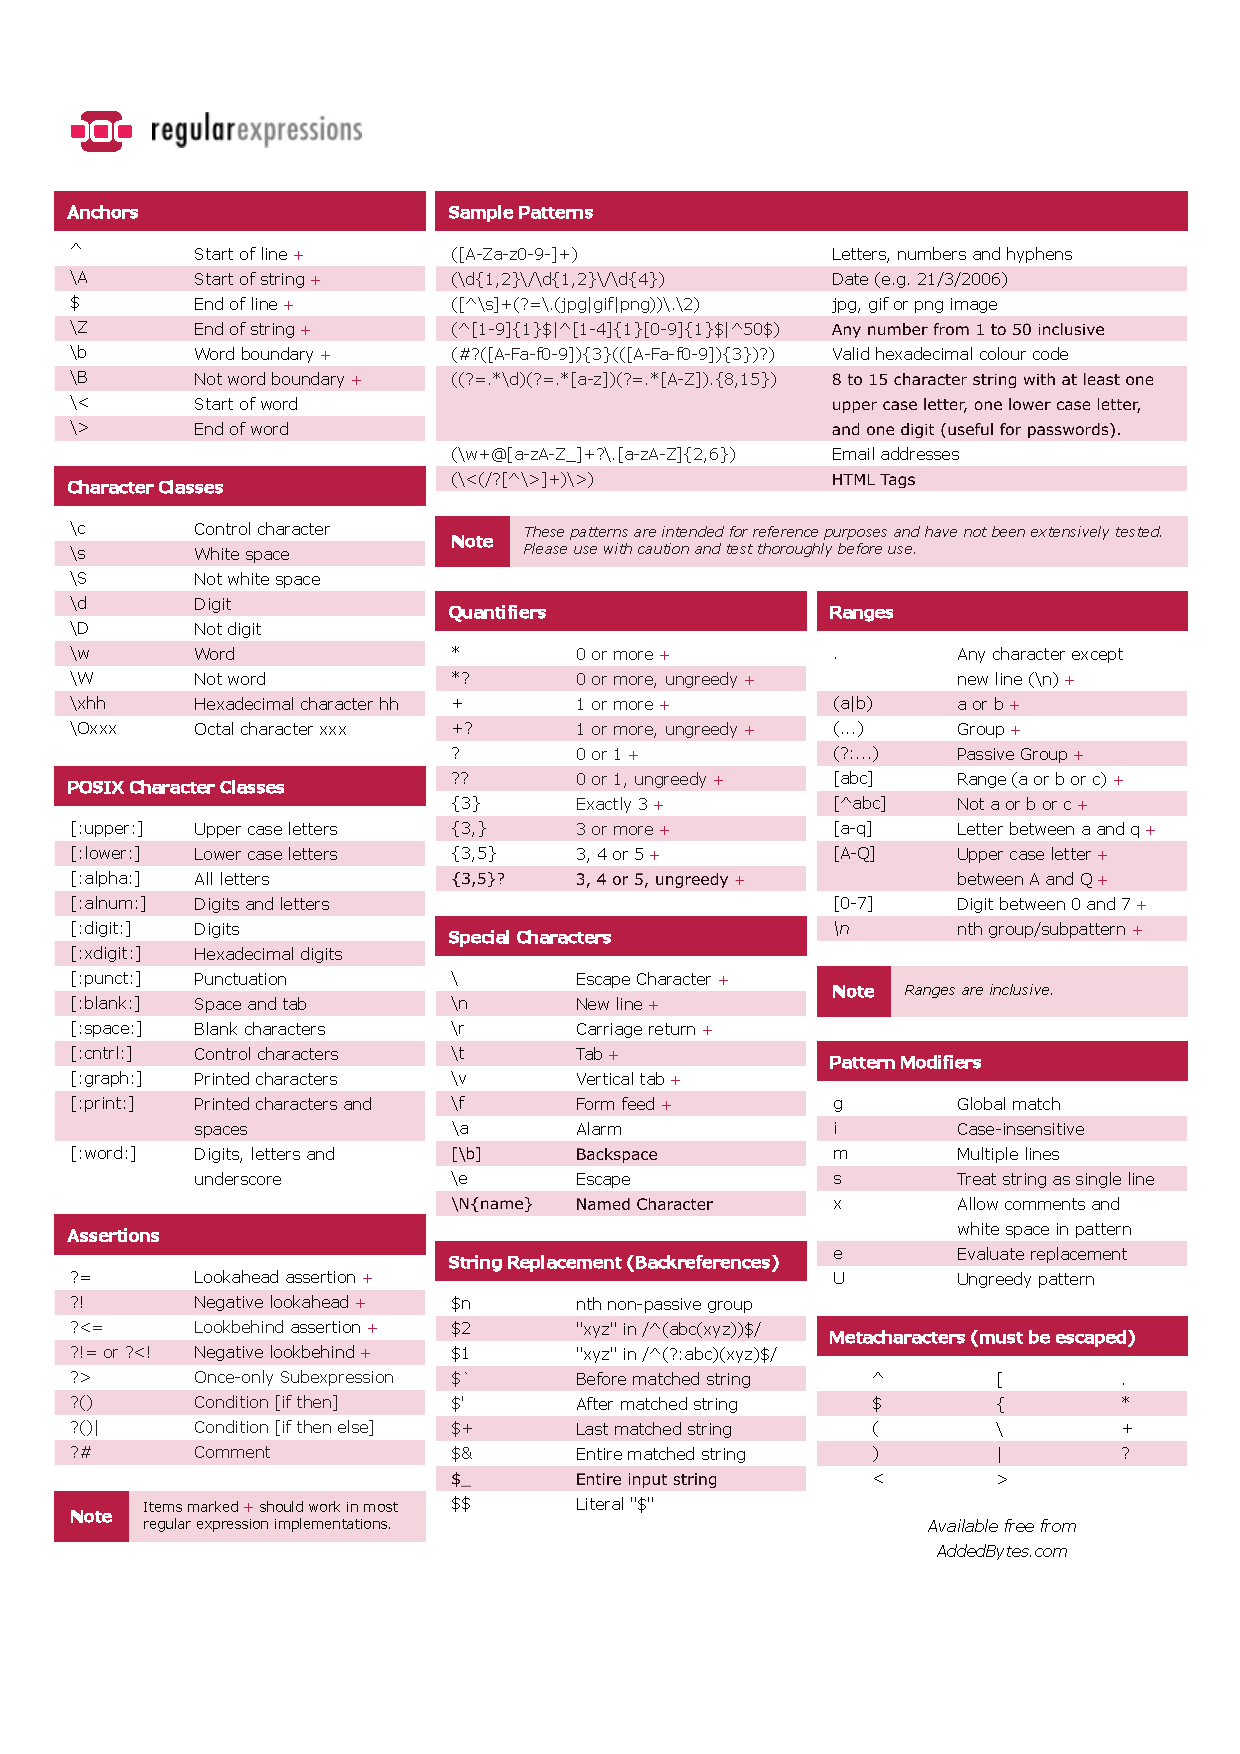
\includepdf[pages={1}]{pdfs/regex.pdf}

\end{document}
